% Chapter 9: ARCH and GARCH models
% Statistics of Financial Markets -- Bachelor's programme, Bucharest University of Economic Studies
% GENERATED by latex/build_chapter9.py -- edit the generator, not this file.

\newcommand{\coursename}{Statistics of Financial Markets}
% Preambul comun SFM -- Statistica piețelor financiare / Statistics of Financial Markets (Beamer, 16:9)
% Același design ca MFM. Înainte de % Preambul comun SFM -- Statistica piețelor financiare / Statistics of Financial Markets (Beamer, 16:9)
% Același design ca MFM. Înainte de % Preambul comun SFM -- Statistica piețelor financiare / Statistics of Financial Markets (Beamer, 16:9)
% Același design ca MFM. Înainte de \input{../../latex/preamble} se definește
%   \newcommand{\coursename}{Statistics of Financial Markets}      (EN)
%   \newcommand{\coursename}{Statistica piețelor financiare}       (RO)  și  \def\sfmlang{ro}
% Fișierele .tex se află în EN/Courses, EN/Seminars, RO/Cursuri, RO/Seminarii (două niveluri sub rădăcină).
% Deck-urile sînt generate de latex/build_chapterN.py / build_seminarN.py (vezi latex/sfm_build.py).

\documentclass[9pt, aspectratio=169, t]{beamer}
\providecommand{\coursename}{Statistics of Financial Markets}

% Ensure content fits on slides
\setbeamersize{text margin left=8mm, text margin right=8mm}

%=============================================================================
% THEME AND STYLE CONFIGURATION
%=============================================================================
\usetheme{default}
% Using default theme for clean header/footer control

% Color Palette (matching Redispatch PDF)
\definecolor{MainBlue}{RGB}{26, 58, 110}
\definecolor{AccentBlue}{RGB}{26, 58, 110}
\definecolor{IDAred}{RGB}{205, 0, 0}
\definecolor{DarkGray}{RGB}{51, 51, 51}
\definecolor{MediumGray}{RGB}{128, 128, 128}
\definecolor{LightGray}{RGB}{248, 248, 248}
\definecolor{VeryLightGray}{RGB}{235, 235, 235}
\definecolor{KeynoteGray}{RGB}{218, 218, 218}
\definecolor{SectionGray}{RGB}{120, 120, 120}
\definecolor{FooterGray}{RGB}{100, 100, 100}
\definecolor{Crimson}{RGB}{220, 53, 69}
\definecolor{Forest}{RGB}{46, 125, 50}
\definecolor{Amber}{RGB}{181, 133, 63}
\definecolor{Orange}{RGB}{230, 126, 34}
\definecolor{Purple}{RGB}{142, 68, 173}

% Gradient background (exact Keynote 315° gradient: white to RGB 218,218,218)
\setbeamertemplate{background}{%
    \begin{tikzpicture}[remember picture, overlay]
        \shade[shading=axis, shading angle=315,
        top color=white, bottom color=KeynoteGray]
        (current page.south west) rectangle (current page.north east);
    \end{tikzpicture}%
}
% Fallback solid color for compatibility
\setbeamercolor{background canvas}{bg=}

\setbeamercolor{palette primary}{bg=MainBlue, fg=white}
\setbeamercolor{palette secondary}{bg=MainBlue!85, fg=white}
\setbeamercolor{palette tertiary}{bg=MainBlue!70, fg=white}
\setbeamercolor{structure}{fg=MainBlue}
\setbeamercolor{title}{fg=IDAred}
\setbeamercolor{frametitle}{fg=IDAred, bg=}
\setbeamercolor{block title}{bg=MainBlue, fg=white}
\setbeamercolor{block body}{bg=VeryLightGray, fg=DarkGray}
\setbeamercolor{block title alerted}{bg=Crimson, fg=white}
\setbeamercolor{block body alerted}{bg=Crimson!8, fg=DarkGray}
\setbeamercolor{block title example}{bg=Forest, fg=white}
\setbeamercolor{block body example}{bg=Forest!8, fg=DarkGray}
\setbeamercolor{item}{fg=MainBlue}

% Footer colors (override Madrid theme blue)
\setbeamercolor{author in head/foot}{fg=FooterGray, bg=}
\setbeamercolor{title in head/foot}{fg=FooterGray, bg=}
\setbeamercolor{date in head/foot}{fg=FooterGray, bg=}
\setbeamercolor{section in head/foot}{fg=FooterGray, bg=}
\setbeamercolor{subsection in head/foot}{fg=FooterGray, bg=}

% Bullet styles (apply everywhere including blocks)
\setbeamertemplate{itemize item}{\color{MainBlue}$\boxdot$}
\setbeamertemplate{itemize subitem}{\color{MainBlue}$\blacktriangleright$}
\setbeamertemplate{itemize subsubitem}{\color{MainBlue}\tiny$\bullet$}
\setbeamertemplate{itemize/enumerate body begin}{\normalsize}
\setbeamertemplate{itemize/enumerate subbody begin}{\normalsize}

% Item spacing - compact style
\setlength{\leftmargini}{10pt}       % Level 1: minimal indent
\setlength{\leftmarginii}{10pt}      % Level 2: minimal additional indent
% Compact list spacing (zero extra space before/after lists in blocks)
\makeatletter
\def\@listi{\leftmargin\leftmargini \topsep 0pt \parsep 0pt \itemsep 0pt}
\def\@listii{\leftmargin\leftmarginii \topsep 0pt \parsep 0pt \itemsep 0pt}
\makeatother

\setbeamertemplate{navigation symbols}{}

%=============================================================================
% CUSTOM HEADLINE
%=============================================================================
\setbeamertemplate{headline}{%
    \vskip10pt%
    \hbox to \paperwidth{%
        \hskip0.5cm%
        {\small\color{FooterGray}\renewcommand{\hyperlink}[2]{##2}\insertsectionhead}%
        \hfill%
        \textcolor{FooterGray}{\small\insertframenumber}%
        \hskip0.5cm%
    }%
    \vskip4pt%
    {\color{FooterGray}\hrule height 0.4pt}%
}

%=============================================================================
% CUSTOM FOOTER
%=============================================================================
\usepackage{fontawesome5}

\setbeamertemplate{footline}{%
    {\color{FooterGray}\hrule height 0.4pt}%
    \vskip4pt%
    \hbox to \paperwidth{%
        \hskip0.5cm%
        \textcolor{FooterGray}{\small\coursename}%
        \hfill%
        \raisebox{-0.1em}{%
            \begin{tikzpicture}[x=0.08em, y=0.08em, line width=0.4pt]
                \draw[FooterGray] (0,3) -- (1,4) -- (2,3.5) -- (3,5) -- (4,4) -- (5,6) -- (6,5.5) -- (7,4) -- (8,5) -- (9,7) -- (10,6) -- (11,5) -- (12,6.5) -- (13,8) -- (14,7) -- (15,6) -- (16,7.5) -- (17,9) -- (18,8) -- (19,7) -- (20,8.5) -- (21,10) -- (22,9) -- (23,8) -- (24,9.5);
            \end{tikzpicture}%
        }%
        \hskip0.5cm%
    }%
    \vskip6pt%
}

%=============================================================================
% PACKAGES
%=============================================================================
\usepackage[utf8]{inputenc}
\DeclareUnicodeCharacter{03B1}{\ensuremath{\alpha}}
\usepackage[T1]{fontenc}
\usepackage{amsmath, amssymb, amsthm}
\usepackage{mathtools}
\usepackage{bm}
\usepackage{tikz}
\usetikzlibrary{arrows.meta, positioning, shapes, calc, decorations.pathreplacing, shadings}
\usepackage{booktabs}
\usepackage{multirow}
\usepackage{array}
\usepackage{graphicx}
\usepackage{hyperref}
\usepackage{colortbl}
\usepackage{listings}
\lstset{language=Python, basicstyle=\ttfamily\scriptsize, keywordstyle=\color{MainBlue}\bfseries,
  commentstyle=\color{Forest}, stringstyle=\color{Crimson}, breaklines=true,
  frame=none, backgroundcolor=\color{VeryLightGray}, xleftmargin=2mm}
\hypersetup{colorlinks=true, linkcolor=MainBlue, urlcolor=MainBlue}
\graphicspath{{../../logos/}{../../charts/}{../../photos/}}
\usepackage{xcolor}
\hfuzz=2pt  % Suppress tiny overfull warnings (<2pt)
\vfuzz=2pt  % Suppress tiny vertical overfull warnings (<2pt)

%=============================================================================
% QUANTLET COMMANDS
%   \quantlet{<displayed name>}{<url>}       (generic, compatible with the older SFM decks)
%   \sfmquantlet{Ch_05}{SFM_ch5_garch}       -> https://github.com/danpele/SFM/tree/main/Quantlets/Ch_05/SFM_ch5_garch
%   \qlurl{<folder>} is defined per chapter by the generator (Quantlets/Ch_NN/<folder>)
%=============================================================================
\newcommand{\sfmrepo}{https://github.com/danpele/SFM}
\newcommand{\sfmqlbase}{https://github.com/danpele/SFM/tree/main/Quantlets}
\newcommand{\quantlet}[2]{%
    \hfill\href{#2}{%
        \raisebox{-0.15em}{
\includegraphics[height=0.7em]{ql_logo.png}}%
        \textcolor{MainBlue}{\tiny\ #1}%
    }%
}
\newcommand{\sfmquantlet}[2]{\quantlet{\detokenize{#2}}{\sfmqlbase/#1/#2}}

%=============================================================================
% NOTEBOOKS (Google Colab)
%   \colaburl{notebooks/EN/chapter5_seminar_notebook.ipynb} -> the Colab link of a file in the SFM repo
%   \nb: the chapter notebook (each seminar deck redefines it with \renewcommand)
%=============================================================================
\newcommand{\colaburl}[1]{https://colab.research.google.com/github/danpele/SFM/blob/main/#1}
\newcommand{\nb}{https://colab.research.google.com/github/danpele/SFM/tree/main/notebooks/EN}
\newcommand{\nbname}{notebooks/EN}

%=============================================================================
% SLIDE HELPERS (used by the generators; the same as in MFM)
%=============================================================================
% local font size for list bodies (the preamble forces \normalsize)
\newcommand{\itemsize}[1]{\setbeamertemplate{itemize/enumerate body begin}{#1}\setbeamertemplate{itemize/enumerate subbody begin}{#1}}
\newcommand{\intitle}[1]{{\hypersetup{urlcolor=white}#1}}   % white links inside coloured title bars
\newcommand{\imgcap}[1]{{\scriptsize #1}\\[0.5mm]}          % caption under a photo
\newcommand{\imgcredit}[2]{{\tiny\color{FooterGray}\href{#1}{#2}}}   % image credit: source URL, author/licence
\newcommand{\aiprompt}[1]{{\ttfamily\color{MainBlue}#1}}     % a prompt to an AI assistant

%=============================================================================
% SEMINARS: student version by default; the instructor wrapper *_solutions.tex sets \solutionstrue
%=============================================================================
\makeatletter\@ifundefined{ifsolutions}{\expandafter\newif\csname ifsolutions\endcsname}{}\makeatother
\newcommand{\solonly}[1]{\ifsolutions #1\fi}
\newcommand{\propsub}{\ifsolutions\else\framesubtitle{\ifdefined\sfmlang Rezolvarea se discută la seminar\else Solution discussed in class\fi}\fi}

%=============================================================================
% APPENDIX AND CHAPTER LINKS (latex/appendix_links.py writes the calls; it also re-declares these
% macros before \begin{document}, so the decks compile with or without this preamble block)
%=============================================================================
\providecommand{\sfmapplink}[3]{\hypertarget{#2}{}\hyperlink{#1}{\beamergotobutton{#3}}}
\providecommand{\sfmappback}[2]{\begin{tikzpicture}[remember picture,overlay]\node[anchor=south east] at ([xshift=-3mm,yshift=7mm]current page.south east){\hyperlink{#1}{\beamerreturnbutton{#2}}};\end{tikzpicture}}
\providecommand{\sfmchlink}[2]{\href{#1}{#2}}
\providecommand{\sfmchlinkt}[2]{\href{#1}{\usebeamercolor[fg]{frametitle}#2}}

%=============================================================================
% QUANTINAR COMMAND: link către un curs Quantinar (subiecte avansate)
%=============================================================================
\newcommand{\quantinar}[2]{%
    \href{#2}{%
        \raisebox{-0.15em}{
\includegraphics[height=0.8em]{qr_logo.png}}%
        \textcolor{MainBlue}{\scriptsize\ #1}%
    }%
}

%=============================================================================
% CUSTOM TITLE PAGE
%=============================================================================
\defbeamertemplate*{title page}{hybrid}[1][]
{
    \vspace{0.2cm}
    % Logos row - top header (with clickable links)
    \begin{center}
        \href{https://www.ase.ro}{
\includegraphics[height=1.0cm]{ase_logo.png}}\hspace{0.3cm}%
        \href{https://theida.net}{
\includegraphics[height=1.0cm]{ida_logo.png}}\hspace{0.3cm}%
        \href{https://blockchain-research-center.com}{
\includegraphics[height=1.0cm]{brc_logo.png}}\hspace{0.3cm}%
        \href{https://www.ai4efin.ase.ro}{
\includegraphics[height=1.0cm]{ai4efin_logo.png}}\hspace{0.3cm}%
        \href{https://ipe.ro/new}{
\includegraphics[height=1.0cm]{acad_logo.png}}\hspace{0.3cm}%
        \href{https://www.digital-finance-msca.com}{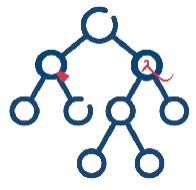
\includegraphics[height=1.0cm]{msca_logo.png}}%
    \end{center}

    \vspace{0.6cm}

    % Main title with Q logos on sides (with clickable links)
    \begin{center}
        \begin{minipage}{0.1\textwidth}
            \centering
            \href{https://quantlet.com}{
\includegraphics[height=1.1cm]{ql_logo.png}}
        \end{minipage}%
        \begin{minipage}{0.78\textwidth}
            \centering
            {\LARGE\bfseries\usebeamercolor[fg]{title}\inserttitle}

            \vspace{0.3cm}

            {\usebeamerfont{subtitle}\usebeamercolor[fg]{title}\insertsubtitle}
        \end{minipage}%
        \begin{minipage}{0.1\textwidth}
            \centering
            \href{https://quantinar.com}{
\includegraphics[height=1.1cm]{qr_logo.png}}
        \end{minipage}
    \end{center}

    \vspace{0.6cm}

    % Authors (left aligned)
    \hspace{0.5cm}{\usebeamerfont{author}\insertauthor}

    \vspace{0.3cm}

    % Institute/Affiliations (left aligned)
    \hspace{0.5cm}\begin{minipage}[t]{0.9\textwidth}
        \raggedright\small\insertinstitute
    \end{minipage}
}

%=============================================================================
% THEOREM ENVIRONMENTS
%=============================================================================
\theoremstyle{definition}
\setbeamertemplate{theorems}[numbered]
\ifdefined\sfmlang
\newtheorem{defn}{Definiție}
\newtheorem{thm}{Teoremă}
\newtheorem{prop}{Propoziție}
\newtheorem{rmk}{Observație}
\else
\newtheorem{defn}{Definition}
\newtheorem{thm}{Theorem}
\newtheorem{prop}{Proposition}
\newtheorem{rmk}{Remark}
\fi

%=============================================================================
% CENTRED MINIPAGE (no extra vertical space)
%=============================================================================
\newenvironment{cminipage}[1]{%
    \par\noindent\hfill\begin{minipage}{#1}\ignorespaces
}{%
    \end{minipage}\hfill\null\par
}

%=============================================================================
% CUSTOM COMMANDS
%=============================================================================
\newcommand{\E}{\mathbb{E}}
\newcommand{\Var}{\text{Var}}
\newcommand{\Cov}{\text{Cov}}
\newcommand{\Corr}{\text{Corr}}
\newcommand{\R}{\mathbb{R}}
\newcommand{\N}{\mathbb{N}}
\newcommand{\Z}{\mathbb{Z}}
\newcommand{\B}{\mathbf{B}}
\newcommand{\imark}{\textcolor{MainBlue}{\textbullet}}
\newcommand{\RMSE}{\text{RMSE}}
\newcommand{\MAE}{\text{MAE}}
\newcommand{\MAPE}{\text{MAPE}}

 se definește
%   \newcommand{\coursename}{Statistics of Financial Markets}      (EN)
%   \newcommand{\coursename}{Statistica piețelor financiare}       (RO)  și  \def\sfmlang{ro}
% Fișierele .tex se află în EN/Courses, EN/Seminars, RO/Cursuri, RO/Seminarii (două niveluri sub rădăcină).
% Deck-urile sînt generate de latex/build_chapterN.py / build_seminarN.py (vezi latex/sfm_build.py).

\documentclass[9pt, aspectratio=169, t]{beamer}
\providecommand{\coursename}{Statistics of Financial Markets}

% Ensure content fits on slides
\setbeamersize{text margin left=8mm, text margin right=8mm}

%=============================================================================
% THEME AND STYLE CONFIGURATION
%=============================================================================
\usetheme{default}
% Using default theme for clean header/footer control

% Color Palette (matching Redispatch PDF)
\definecolor{MainBlue}{RGB}{26, 58, 110}
\definecolor{AccentBlue}{RGB}{26, 58, 110}
\definecolor{IDAred}{RGB}{205, 0, 0}
\definecolor{DarkGray}{RGB}{51, 51, 51}
\definecolor{MediumGray}{RGB}{128, 128, 128}
\definecolor{LightGray}{RGB}{248, 248, 248}
\definecolor{VeryLightGray}{RGB}{235, 235, 235}
\definecolor{KeynoteGray}{RGB}{218, 218, 218}
\definecolor{SectionGray}{RGB}{120, 120, 120}
\definecolor{FooterGray}{RGB}{100, 100, 100}
\definecolor{Crimson}{RGB}{220, 53, 69}
\definecolor{Forest}{RGB}{46, 125, 50}
\definecolor{Amber}{RGB}{181, 133, 63}
\definecolor{Orange}{RGB}{230, 126, 34}
\definecolor{Purple}{RGB}{142, 68, 173}

% Gradient background (exact Keynote 315° gradient: white to RGB 218,218,218)
\setbeamertemplate{background}{%
    \begin{tikzpicture}[remember picture, overlay]
        \shade[shading=axis, shading angle=315,
        top color=white, bottom color=KeynoteGray]
        (current page.south west) rectangle (current page.north east);
    \end{tikzpicture}%
}
% Fallback solid color for compatibility
\setbeamercolor{background canvas}{bg=}

\setbeamercolor{palette primary}{bg=MainBlue, fg=white}
\setbeamercolor{palette secondary}{bg=MainBlue!85, fg=white}
\setbeamercolor{palette tertiary}{bg=MainBlue!70, fg=white}
\setbeamercolor{structure}{fg=MainBlue}
\setbeamercolor{title}{fg=IDAred}
\setbeamercolor{frametitle}{fg=IDAred, bg=}
\setbeamercolor{block title}{bg=MainBlue, fg=white}
\setbeamercolor{block body}{bg=VeryLightGray, fg=DarkGray}
\setbeamercolor{block title alerted}{bg=Crimson, fg=white}
\setbeamercolor{block body alerted}{bg=Crimson!8, fg=DarkGray}
\setbeamercolor{block title example}{bg=Forest, fg=white}
\setbeamercolor{block body example}{bg=Forest!8, fg=DarkGray}
\setbeamercolor{item}{fg=MainBlue}

% Footer colors (override Madrid theme blue)
\setbeamercolor{author in head/foot}{fg=FooterGray, bg=}
\setbeamercolor{title in head/foot}{fg=FooterGray, bg=}
\setbeamercolor{date in head/foot}{fg=FooterGray, bg=}
\setbeamercolor{section in head/foot}{fg=FooterGray, bg=}
\setbeamercolor{subsection in head/foot}{fg=FooterGray, bg=}

% Bullet styles (apply everywhere including blocks)
\setbeamertemplate{itemize item}{\color{MainBlue}$\boxdot$}
\setbeamertemplate{itemize subitem}{\color{MainBlue}$\blacktriangleright$}
\setbeamertemplate{itemize subsubitem}{\color{MainBlue}\tiny$\bullet$}
\setbeamertemplate{itemize/enumerate body begin}{\normalsize}
\setbeamertemplate{itemize/enumerate subbody begin}{\normalsize}

% Item spacing - compact style
\setlength{\leftmargini}{10pt}       % Level 1: minimal indent
\setlength{\leftmarginii}{10pt}      % Level 2: minimal additional indent
% Compact list spacing (zero extra space before/after lists in blocks)
\makeatletter
\def\@listi{\leftmargin\leftmargini \topsep 0pt \parsep 0pt \itemsep 0pt}
\def\@listii{\leftmargin\leftmarginii \topsep 0pt \parsep 0pt \itemsep 0pt}
\makeatother

\setbeamertemplate{navigation symbols}{}

%=============================================================================
% CUSTOM HEADLINE
%=============================================================================
\setbeamertemplate{headline}{%
    \vskip10pt%
    \hbox to \paperwidth{%
        \hskip0.5cm%
        {\small\color{FooterGray}\renewcommand{\hyperlink}[2]{##2}\insertsectionhead}%
        \hfill%
        \textcolor{FooterGray}{\small\insertframenumber}%
        \hskip0.5cm%
    }%
    \vskip4pt%
    {\color{FooterGray}\hrule height 0.4pt}%
}

%=============================================================================
% CUSTOM FOOTER
%=============================================================================
\usepackage{fontawesome5}

\setbeamertemplate{footline}{%
    {\color{FooterGray}\hrule height 0.4pt}%
    \vskip4pt%
    \hbox to \paperwidth{%
        \hskip0.5cm%
        \textcolor{FooterGray}{\small\coursename}%
        \hfill%
        \raisebox{-0.1em}{%
            \begin{tikzpicture}[x=0.08em, y=0.08em, line width=0.4pt]
                \draw[FooterGray] (0,3) -- (1,4) -- (2,3.5) -- (3,5) -- (4,4) -- (5,6) -- (6,5.5) -- (7,4) -- (8,5) -- (9,7) -- (10,6) -- (11,5) -- (12,6.5) -- (13,8) -- (14,7) -- (15,6) -- (16,7.5) -- (17,9) -- (18,8) -- (19,7) -- (20,8.5) -- (21,10) -- (22,9) -- (23,8) -- (24,9.5);
            \end{tikzpicture}%
        }%
        \hskip0.5cm%
    }%
    \vskip6pt%
}

%=============================================================================
% PACKAGES
%=============================================================================
\usepackage[utf8]{inputenc}
\DeclareUnicodeCharacter{03B1}{\ensuremath{\alpha}}
\usepackage[T1]{fontenc}
\usepackage{amsmath, amssymb, amsthm}
\usepackage{mathtools}
\usepackage{bm}
\usepackage{tikz}
\usetikzlibrary{arrows.meta, positioning, shapes, calc, decorations.pathreplacing, shadings}
\usepackage{booktabs}
\usepackage{multirow}
\usepackage{array}
\usepackage{graphicx}
\usepackage{hyperref}
\usepackage{colortbl}
\usepackage{listings}
\lstset{language=Python, basicstyle=\ttfamily\scriptsize, keywordstyle=\color{MainBlue}\bfseries,
  commentstyle=\color{Forest}, stringstyle=\color{Crimson}, breaklines=true,
  frame=none, backgroundcolor=\color{VeryLightGray}, xleftmargin=2mm}
\hypersetup{colorlinks=true, linkcolor=MainBlue, urlcolor=MainBlue}
\graphicspath{{../../logos/}{../../charts/}{../../photos/}}
\usepackage{xcolor}
\hfuzz=2pt  % Suppress tiny overfull warnings (<2pt)
\vfuzz=2pt  % Suppress tiny vertical overfull warnings (<2pt)

%=============================================================================
% QUANTLET COMMANDS
%   \quantlet{<displayed name>}{<url>}       (generic, compatible with the older SFM decks)
%   \sfmquantlet{Ch_05}{SFM_ch5_garch}       -> https://github.com/danpele/SFM/tree/main/Quantlets/Ch_05/SFM_ch5_garch
%   \qlurl{<folder>} is defined per chapter by the generator (Quantlets/Ch_NN/<folder>)
%=============================================================================
\newcommand{\sfmrepo}{https://github.com/danpele/SFM}
\newcommand{\sfmqlbase}{https://github.com/danpele/SFM/tree/main/Quantlets}
\newcommand{\quantlet}[2]{%
    \hfill\href{#2}{%
        \raisebox{-0.15em}{
\includegraphics[height=0.7em]{ql_logo.png}}%
        \textcolor{MainBlue}{\tiny\ #1}%
    }%
}
\newcommand{\sfmquantlet}[2]{\quantlet{\detokenize{#2}}{\sfmqlbase/#1/#2}}

%=============================================================================
% NOTEBOOKS (Google Colab)
%   \colaburl{notebooks/EN/chapter5_seminar_notebook.ipynb} -> the Colab link of a file in the SFM repo
%   \nb: the chapter notebook (each seminar deck redefines it with \renewcommand)
%=============================================================================
\newcommand{\colaburl}[1]{https://colab.research.google.com/github/danpele/SFM/blob/main/#1}
\newcommand{\nb}{https://colab.research.google.com/github/danpele/SFM/tree/main/notebooks/EN}
\newcommand{\nbname}{notebooks/EN}

%=============================================================================
% SLIDE HELPERS (used by the generators; the same as in MFM)
%=============================================================================
% local font size for list bodies (the preamble forces \normalsize)
\newcommand{\itemsize}[1]{\setbeamertemplate{itemize/enumerate body begin}{#1}\setbeamertemplate{itemize/enumerate subbody begin}{#1}}
\newcommand{\intitle}[1]{{\hypersetup{urlcolor=white}#1}}   % white links inside coloured title bars
\newcommand{\imgcap}[1]{{\scriptsize #1}\\[0.5mm]}          % caption under a photo
\newcommand{\imgcredit}[2]{{\tiny\color{FooterGray}\href{#1}{#2}}}   % image credit: source URL, author/licence
\newcommand{\aiprompt}[1]{{\ttfamily\color{MainBlue}#1}}     % a prompt to an AI assistant

%=============================================================================
% SEMINARS: student version by default; the instructor wrapper *_solutions.tex sets \solutionstrue
%=============================================================================
\makeatletter\@ifundefined{ifsolutions}{\expandafter\newif\csname ifsolutions\endcsname}{}\makeatother
\newcommand{\solonly}[1]{\ifsolutions #1\fi}
\newcommand{\propsub}{\ifsolutions\else\framesubtitle{\ifdefined\sfmlang Rezolvarea se discută la seminar\else Solution discussed in class\fi}\fi}

%=============================================================================
% APPENDIX AND CHAPTER LINKS (latex/appendix_links.py writes the calls; it also re-declares these
% macros before \begin{document}, so the decks compile with or without this preamble block)
%=============================================================================
\providecommand{\sfmapplink}[3]{\hypertarget{#2}{}\hyperlink{#1}{\beamergotobutton{#3}}}
\providecommand{\sfmappback}[2]{\begin{tikzpicture}[remember picture,overlay]\node[anchor=south east] at ([xshift=-3mm,yshift=7mm]current page.south east){\hyperlink{#1}{\beamerreturnbutton{#2}}};\end{tikzpicture}}
\providecommand{\sfmchlink}[2]{\href{#1}{#2}}
\providecommand{\sfmchlinkt}[2]{\href{#1}{\usebeamercolor[fg]{frametitle}#2}}

%=============================================================================
% QUANTINAR COMMAND: link către un curs Quantinar (subiecte avansate)
%=============================================================================
\newcommand{\quantinar}[2]{%
    \href{#2}{%
        \raisebox{-0.15em}{
\includegraphics[height=0.8em]{qr_logo.png}}%
        \textcolor{MainBlue}{\scriptsize\ #1}%
    }%
}

%=============================================================================
% CUSTOM TITLE PAGE
%=============================================================================
\defbeamertemplate*{title page}{hybrid}[1][]
{
    \vspace{0.2cm}
    % Logos row - top header (with clickable links)
    \begin{center}
        \href{https://www.ase.ro}{
\includegraphics[height=1.0cm]{ase_logo.png}}\hspace{0.3cm}%
        \href{https://theida.net}{
\includegraphics[height=1.0cm]{ida_logo.png}}\hspace{0.3cm}%
        \href{https://blockchain-research-center.com}{
\includegraphics[height=1.0cm]{brc_logo.png}}\hspace{0.3cm}%
        \href{https://www.ai4efin.ase.ro}{
\includegraphics[height=1.0cm]{ai4efin_logo.png}}\hspace{0.3cm}%
        \href{https://ipe.ro/new}{
\includegraphics[height=1.0cm]{acad_logo.png}}\hspace{0.3cm}%
        \href{https://www.digital-finance-msca.com}{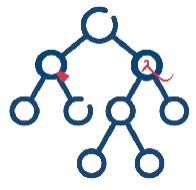
\includegraphics[height=1.0cm]{msca_logo.png}}%
    \end{center}

    \vspace{0.6cm}

    % Main title with Q logos on sides (with clickable links)
    \begin{center}
        \begin{minipage}{0.1\textwidth}
            \centering
            \href{https://quantlet.com}{
\includegraphics[height=1.1cm]{ql_logo.png}}
        \end{minipage}%
        \begin{minipage}{0.78\textwidth}
            \centering
            {\LARGE\bfseries\usebeamercolor[fg]{title}\inserttitle}

            \vspace{0.3cm}

            {\usebeamerfont{subtitle}\usebeamercolor[fg]{title}\insertsubtitle}
        \end{minipage}%
        \begin{minipage}{0.1\textwidth}
            \centering
            \href{https://quantinar.com}{
\includegraphics[height=1.1cm]{qr_logo.png}}
        \end{minipage}
    \end{center}

    \vspace{0.6cm}

    % Authors (left aligned)
    \hspace{0.5cm}{\usebeamerfont{author}\insertauthor}

    \vspace{0.3cm}

    % Institute/Affiliations (left aligned)
    \hspace{0.5cm}\begin{minipage}[t]{0.9\textwidth}
        \raggedright\small\insertinstitute
    \end{minipage}
}

%=============================================================================
% THEOREM ENVIRONMENTS
%=============================================================================
\theoremstyle{definition}
\setbeamertemplate{theorems}[numbered]
\ifdefined\sfmlang
\newtheorem{defn}{Definiție}
\newtheorem{thm}{Teoremă}
\newtheorem{prop}{Propoziție}
\newtheorem{rmk}{Observație}
\else
\newtheorem{defn}{Definition}
\newtheorem{thm}{Theorem}
\newtheorem{prop}{Proposition}
\newtheorem{rmk}{Remark}
\fi

%=============================================================================
% CENTRED MINIPAGE (no extra vertical space)
%=============================================================================
\newenvironment{cminipage}[1]{%
    \par\noindent\hfill\begin{minipage}{#1}\ignorespaces
}{%
    \end{minipage}\hfill\null\par
}

%=============================================================================
% CUSTOM COMMANDS
%=============================================================================
\newcommand{\E}{\mathbb{E}}
\newcommand{\Var}{\text{Var}}
\newcommand{\Cov}{\text{Cov}}
\newcommand{\Corr}{\text{Corr}}
\newcommand{\R}{\mathbb{R}}
\newcommand{\N}{\mathbb{N}}
\newcommand{\Z}{\mathbb{Z}}
\newcommand{\B}{\mathbf{B}}
\newcommand{\imark}{\textcolor{MainBlue}{\textbullet}}
\newcommand{\RMSE}{\text{RMSE}}
\newcommand{\MAE}{\text{MAE}}
\newcommand{\MAPE}{\text{MAPE}}

 se definește
%   \newcommand{\coursename}{Statistics of Financial Markets}      (EN)
%   \newcommand{\coursename}{Statistica piețelor financiare}       (RO)  și  \def\sfmlang{ro}
% Fișierele .tex se află în EN/Courses, EN/Seminars, RO/Cursuri, RO/Seminarii (două niveluri sub rădăcină).
% Deck-urile sînt generate de latex/build_chapterN.py / build_seminarN.py (vezi latex/sfm_build.py).

\documentclass[9pt, aspectratio=169, t]{beamer}
\providecommand{\coursename}{Statistics of Financial Markets}

% Ensure content fits on slides
\setbeamersize{text margin left=8mm, text margin right=8mm}

%=============================================================================
% THEME AND STYLE CONFIGURATION
%=============================================================================
\usetheme{default}
% Using default theme for clean header/footer control

% Color Palette (matching Redispatch PDF)
\definecolor{MainBlue}{RGB}{26, 58, 110}
\definecolor{AccentBlue}{RGB}{26, 58, 110}
\definecolor{IDAred}{RGB}{205, 0, 0}
\definecolor{DarkGray}{RGB}{51, 51, 51}
\definecolor{MediumGray}{RGB}{128, 128, 128}
\definecolor{LightGray}{RGB}{248, 248, 248}
\definecolor{VeryLightGray}{RGB}{235, 235, 235}
\definecolor{KeynoteGray}{RGB}{218, 218, 218}
\definecolor{SectionGray}{RGB}{120, 120, 120}
\definecolor{FooterGray}{RGB}{100, 100, 100}
\definecolor{Crimson}{RGB}{220, 53, 69}
\definecolor{Forest}{RGB}{46, 125, 50}
\definecolor{Amber}{RGB}{181, 133, 63}
\definecolor{Orange}{RGB}{230, 126, 34}
\definecolor{Purple}{RGB}{142, 68, 173}

% Gradient background (exact Keynote 315° gradient: white to RGB 218,218,218)
\setbeamertemplate{background}{%
    \begin{tikzpicture}[remember picture, overlay]
        \shade[shading=axis, shading angle=315,
        top color=white, bottom color=KeynoteGray]
        (current page.south west) rectangle (current page.north east);
    \end{tikzpicture}%
}
% Fallback solid color for compatibility
\setbeamercolor{background canvas}{bg=}

\setbeamercolor{palette primary}{bg=MainBlue, fg=white}
\setbeamercolor{palette secondary}{bg=MainBlue!85, fg=white}
\setbeamercolor{palette tertiary}{bg=MainBlue!70, fg=white}
\setbeamercolor{structure}{fg=MainBlue}
\setbeamercolor{title}{fg=IDAred}
\setbeamercolor{frametitle}{fg=IDAred, bg=}
\setbeamercolor{block title}{bg=MainBlue, fg=white}
\setbeamercolor{block body}{bg=VeryLightGray, fg=DarkGray}
\setbeamercolor{block title alerted}{bg=Crimson, fg=white}
\setbeamercolor{block body alerted}{bg=Crimson!8, fg=DarkGray}
\setbeamercolor{block title example}{bg=Forest, fg=white}
\setbeamercolor{block body example}{bg=Forest!8, fg=DarkGray}
\setbeamercolor{item}{fg=MainBlue}

% Footer colors (override Madrid theme blue)
\setbeamercolor{author in head/foot}{fg=FooterGray, bg=}
\setbeamercolor{title in head/foot}{fg=FooterGray, bg=}
\setbeamercolor{date in head/foot}{fg=FooterGray, bg=}
\setbeamercolor{section in head/foot}{fg=FooterGray, bg=}
\setbeamercolor{subsection in head/foot}{fg=FooterGray, bg=}

% Bullet styles (apply everywhere including blocks)
\setbeamertemplate{itemize item}{\color{MainBlue}$\boxdot$}
\setbeamertemplate{itemize subitem}{\color{MainBlue}$\blacktriangleright$}
\setbeamertemplate{itemize subsubitem}{\color{MainBlue}\tiny$\bullet$}
\setbeamertemplate{itemize/enumerate body begin}{\normalsize}
\setbeamertemplate{itemize/enumerate subbody begin}{\normalsize}

% Item spacing - compact style
\setlength{\leftmargini}{10pt}       % Level 1: minimal indent
\setlength{\leftmarginii}{10pt}      % Level 2: minimal additional indent
% Compact list spacing (zero extra space before/after lists in blocks)
\makeatletter
\def\@listi{\leftmargin\leftmargini \topsep 0pt \parsep 0pt \itemsep 0pt}
\def\@listii{\leftmargin\leftmarginii \topsep 0pt \parsep 0pt \itemsep 0pt}
\makeatother

\setbeamertemplate{navigation symbols}{}

%=============================================================================
% CUSTOM HEADLINE
%=============================================================================
\setbeamertemplate{headline}{%
    \vskip10pt%
    \hbox to \paperwidth{%
        \hskip0.5cm%
        {\small\color{FooterGray}\renewcommand{\hyperlink}[2]{##2}\insertsectionhead}%
        \hfill%
        \textcolor{FooterGray}{\small\insertframenumber}%
        \hskip0.5cm%
    }%
    \vskip4pt%
    {\color{FooterGray}\hrule height 0.4pt}%
}

%=============================================================================
% CUSTOM FOOTER
%=============================================================================
\usepackage{fontawesome5}

\setbeamertemplate{footline}{%
    {\color{FooterGray}\hrule height 0.4pt}%
    \vskip4pt%
    \hbox to \paperwidth{%
        \hskip0.5cm%
        \textcolor{FooterGray}{\small\coursename}%
        \hfill%
        \raisebox{-0.1em}{%
            \begin{tikzpicture}[x=0.08em, y=0.08em, line width=0.4pt]
                \draw[FooterGray] (0,3) -- (1,4) -- (2,3.5) -- (3,5) -- (4,4) -- (5,6) -- (6,5.5) -- (7,4) -- (8,5) -- (9,7) -- (10,6) -- (11,5) -- (12,6.5) -- (13,8) -- (14,7) -- (15,6) -- (16,7.5) -- (17,9) -- (18,8) -- (19,7) -- (20,8.5) -- (21,10) -- (22,9) -- (23,8) -- (24,9.5);
            \end{tikzpicture}%
        }%
        \hskip0.5cm%
    }%
    \vskip6pt%
}

%=============================================================================
% PACKAGES
%=============================================================================
\usepackage[utf8]{inputenc}
\DeclareUnicodeCharacter{03B1}{\ensuremath{\alpha}}
\usepackage[T1]{fontenc}
\usepackage{amsmath, amssymb, amsthm}
\usepackage{mathtools}
\usepackage{bm}
\usepackage{tikz}
\usetikzlibrary{arrows.meta, positioning, shapes, calc, decorations.pathreplacing, shadings}
\usepackage{booktabs}
\usepackage{multirow}
\usepackage{array}
\usepackage{graphicx}
\usepackage{hyperref}
\usepackage{colortbl}
\usepackage{listings}
\lstset{language=Python, basicstyle=\ttfamily\scriptsize, keywordstyle=\color{MainBlue}\bfseries,
  commentstyle=\color{Forest}, stringstyle=\color{Crimson}, breaklines=true,
  frame=none, backgroundcolor=\color{VeryLightGray}, xleftmargin=2mm}
\hypersetup{colorlinks=true, linkcolor=MainBlue, urlcolor=MainBlue}
\graphicspath{{../../logos/}{../../charts/}{../../photos/}}
\usepackage{xcolor}
\hfuzz=2pt  % Suppress tiny overfull warnings (<2pt)
\vfuzz=2pt  % Suppress tiny vertical overfull warnings (<2pt)

%=============================================================================
% QUANTLET COMMANDS
%   \quantlet{<displayed name>}{<url>}       (generic, compatible with the older SFM decks)
%   \sfmquantlet{Ch_05}{SFM_ch5_garch}       -> https://github.com/danpele/SFM/tree/main/Quantlets/Ch_05/SFM_ch5_garch
%   \qlurl{<folder>} is defined per chapter by the generator (Quantlets/Ch_NN/<folder>)
%=============================================================================
\newcommand{\sfmrepo}{https://github.com/danpele/SFM}
\newcommand{\sfmqlbase}{https://github.com/danpele/SFM/tree/main/Quantlets}
\newcommand{\quantlet}[2]{%
    \hfill\href{#2}{%
        \raisebox{-0.15em}{
\includegraphics[height=0.7em]{ql_logo.png}}%
        \textcolor{MainBlue}{\tiny\ #1}%
    }%
}
\newcommand{\sfmquantlet}[2]{\quantlet{\detokenize{#2}}{\sfmqlbase/#1/#2}}

%=============================================================================
% NOTEBOOKS (Google Colab)
%   \colaburl{notebooks/EN/chapter5_seminar_notebook.ipynb} -> the Colab link of a file in the SFM repo
%   \nb: the chapter notebook (each seminar deck redefines it with \renewcommand)
%=============================================================================
\newcommand{\colaburl}[1]{https://colab.research.google.com/github/danpele/SFM/blob/main/#1}
\newcommand{\nb}{https://colab.research.google.com/github/danpele/SFM/tree/main/notebooks/EN}
\newcommand{\nbname}{notebooks/EN}

%=============================================================================
% SLIDE HELPERS (used by the generators; the same as in MFM)
%=============================================================================
% local font size for list bodies (the preamble forces \normalsize)
\newcommand{\itemsize}[1]{\setbeamertemplate{itemize/enumerate body begin}{#1}\setbeamertemplate{itemize/enumerate subbody begin}{#1}}
\newcommand{\intitle}[1]{{\hypersetup{urlcolor=white}#1}}   % white links inside coloured title bars
\newcommand{\imgcap}[1]{{\scriptsize #1}\\[0.5mm]}          % caption under a photo
\newcommand{\imgcredit}[2]{{\tiny\color{FooterGray}\href{#1}{#2}}}   % image credit: source URL, author/licence
\newcommand{\aiprompt}[1]{{\ttfamily\color{MainBlue}#1}}     % a prompt to an AI assistant

%=============================================================================
% SEMINARS: student version by default; the instructor wrapper *_solutions.tex sets \solutionstrue
%=============================================================================
\makeatletter\@ifundefined{ifsolutions}{\expandafter\newif\csname ifsolutions\endcsname}{}\makeatother
\newcommand{\solonly}[1]{\ifsolutions #1\fi}
\newcommand{\propsub}{\ifsolutions\else\framesubtitle{\ifdefined\sfmlang Rezolvarea se discută la seminar\else Solution discussed in class\fi}\fi}

%=============================================================================
% APPENDIX AND CHAPTER LINKS (latex/appendix_links.py writes the calls; it also re-declares these
% macros before \begin{document}, so the decks compile with or without this preamble block)
%=============================================================================
\providecommand{\sfmapplink}[3]{\hypertarget{#2}{}\hyperlink{#1}{\beamergotobutton{#3}}}
\providecommand{\sfmappback}[2]{\begin{tikzpicture}[remember picture,overlay]\node[anchor=south east] at ([xshift=-3mm,yshift=7mm]current page.south east){\hyperlink{#1}{\beamerreturnbutton{#2}}};\end{tikzpicture}}
\providecommand{\sfmchlink}[2]{\href{#1}{#2}}
\providecommand{\sfmchlinkt}[2]{\href{#1}{\usebeamercolor[fg]{frametitle}#2}}

%=============================================================================
% QUANTINAR COMMAND: link către un curs Quantinar (subiecte avansate)
%=============================================================================
\newcommand{\quantinar}[2]{%
    \href{#2}{%
        \raisebox{-0.15em}{
\includegraphics[height=0.8em]{qr_logo.png}}%
        \textcolor{MainBlue}{\scriptsize\ #1}%
    }%
}

%=============================================================================
% CUSTOM TITLE PAGE
%=============================================================================
\defbeamertemplate*{title page}{hybrid}[1][]
{
    \vspace{0.2cm}
    % Logos row - top header (with clickable links)
    \begin{center}
        \href{https://www.ase.ro}{
\includegraphics[height=1.0cm]{ase_logo.png}}\hspace{0.3cm}%
        \href{https://theida.net}{
\includegraphics[height=1.0cm]{ida_logo.png}}\hspace{0.3cm}%
        \href{https://blockchain-research-center.com}{
\includegraphics[height=1.0cm]{brc_logo.png}}\hspace{0.3cm}%
        \href{https://www.ai4efin.ase.ro}{
\includegraphics[height=1.0cm]{ai4efin_logo.png}}\hspace{0.3cm}%
        \href{https://ipe.ro/new}{
\includegraphics[height=1.0cm]{acad_logo.png}}\hspace{0.3cm}%
        \href{https://www.digital-finance-msca.com}{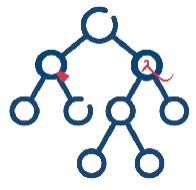
\includegraphics[height=1.0cm]{msca_logo.png}}%
    \end{center}

    \vspace{0.6cm}

    % Main title with Q logos on sides (with clickable links)
    \begin{center}
        \begin{minipage}{0.1\textwidth}
            \centering
            \href{https://quantlet.com}{
\includegraphics[height=1.1cm]{ql_logo.png}}
        \end{minipage}%
        \begin{minipage}{0.78\textwidth}
            \centering
            {\LARGE\bfseries\usebeamercolor[fg]{title}\inserttitle}

            \vspace{0.3cm}

            {\usebeamerfont{subtitle}\usebeamercolor[fg]{title}\insertsubtitle}
        \end{minipage}%
        \begin{minipage}{0.1\textwidth}
            \centering
            \href{https://quantinar.com}{
\includegraphics[height=1.1cm]{qr_logo.png}}
        \end{minipage}
    \end{center}

    \vspace{0.6cm}

    % Authors (left aligned)
    \hspace{0.5cm}{\usebeamerfont{author}\insertauthor}

    \vspace{0.3cm}

    % Institute/Affiliations (left aligned)
    \hspace{0.5cm}\begin{minipage}[t]{0.9\textwidth}
        \raggedright\small\insertinstitute
    \end{minipage}
}

%=============================================================================
% THEOREM ENVIRONMENTS
%=============================================================================
\theoremstyle{definition}
\setbeamertemplate{theorems}[numbered]
\ifdefined\sfmlang
\newtheorem{defn}{Definiție}
\newtheorem{thm}{Teoremă}
\newtheorem{prop}{Propoziție}
\newtheorem{rmk}{Observație}
\else
\newtheorem{defn}{Definition}
\newtheorem{thm}{Theorem}
\newtheorem{prop}{Proposition}
\newtheorem{rmk}{Remark}
\fi

%=============================================================================
% CENTRED MINIPAGE (no extra vertical space)
%=============================================================================
\newenvironment{cminipage}[1]{%
    \par\noindent\hfill\begin{minipage}{#1}\ignorespaces
}{%
    \end{minipage}\hfill\null\par
}

%=============================================================================
% CUSTOM COMMANDS
%=============================================================================
\newcommand{\E}{\mathbb{E}}
\newcommand{\Var}{\text{Var}}
\newcommand{\Cov}{\text{Cov}}
\newcommand{\Corr}{\text{Corr}}
\newcommand{\R}{\mathbb{R}}
\newcommand{\N}{\mathbb{N}}
\newcommand{\Z}{\mathbb{Z}}
\newcommand{\B}{\mathbf{B}}
\newcommand{\imark}{\textcolor{MainBlue}{\textbullet}}
\newcommand{\RMSE}{\text{RMSE}}
\newcommand{\MAE}{\text{MAE}}
\newcommand{\MAPE}{\text{MAPE}}



\newcommand{\qlurl}[1]{https://github.com/danpele/SFM/tree/main/Quantlets/Ch_09/#1}

% Clickable citations (DOIs verified via Crossref)

\newcommand{\refEngle}{\href{https://doi.org/10.2307/1912773}{Engle (1982)}}
\newcommand{\refBoll}{\href{https://doi.org/10.1016/0304-4076(86)90063-1}{Bollerslev (1986)}}
\newcommand{\refBollT}{\href{https://doi.org/10.2307/1925546}{Bollerslev (1987)}}
\newcommand{\refEB}{\href{https://doi.org/10.1080/07474938608800095}{Engle \& Bollerslev (1986)}}
\newcommand{\refNelson}{\href{https://doi.org/10.2307/2938260}{Nelson (1991)}}
\newcommand{\refGJR}{\href{https://doi.org/10.1111/j.1540-6261.1993.tb05128.x}{Glosten, Jagannathan \& Runkle (1993)}}
\newcommand{\refEN}{\href{https://doi.org/10.1111/j.1540-6261.1993.tb05127.x}{Engle \& Ng (1993)}}
\newcommand{\refBW}{\href{https://doi.org/10.1080/07474939208800229}{Bollerslev \& Wooldridge (1992)}}
\newcommand{\refHansen}{\href{https://doi.org/10.2307/2527081}{Hansen (1994)}}
\newcommand{\refPatton}{\href{https://doi.org/10.1016/j.jeconom.2010.03.034}{Patton (2011)}}
\newcommand{\refHL}{\href{https://doi.org/10.1002/jae.800}{Hansen \& Lunde (2005)}}
\newcommand{\refAB}{\href{https://doi.org/10.2307/2527343}{Andersen \& Bollerslev (1998)}}
\newcommand{\refChristie}{\href{https://doi.org/10.1016/0304-405X(82)90018-6}{Christie (1982)}}
\newcommand{\refEngleN}{\href{https://doi.org/10.1257/0002828041464597}{Engle (2004)}}
\newcommand{\refDM}{\href{https://doi.org/10.1080/07350015.1995.10524599}{Diebold \& Mariano (1995)}}
\newcommand{\refAkaike}{\href{https://doi.org/10.1109/TAC.1974.1100705}{Akaike (1974)}}
\newcommand{\refSchwarz}{\href{https://doi.org/10.1214/aos/1176344136}{Schwarz (1978)}}
\newcommand{\refKupiec}{\href{https://doi.org/10.3905/jod.1995.407942}{Kupiec (1995)}}
\newcommand{\refLjung}{\href{https://doi.org/10.1093/biomet/65.2.297}{Ljung \& Box (1978)}}
\newcommand{\refFHH}{\href{https://doi.org/10.1007/978-3-030-13751-9}{Franke, Härdle \& Hafner (2019)}}
\newcommand{\refBHL}{\href{https://doi.org/10.1007/978-3-642-33929-5}{Borak, Härdle \& López-Cabrera (2013)}}
\newcommand{\refTsay}{\href{https://doi.org/10.1002/9780470644560}{Tsay (2010)}}
\newcommand{\refWang}{\href{https://doi.org/10.1038/s41586-023-06221-2}{Wang et al.\ (2023)}}
\newcommand{\refPeleA}{\href{https://doi.org/10.3390/e19050226}{Pele, Lazar \& Dufour (2017)}}
\newcommand{\refPeleB}{\href{https://doi.org/10.3390/e21020102}{Pele \& Mazurencu-Marinescu-Pele (2019)}}
\newcommand{\refPeleC}{\href{https://doi.org/10.1080/1351847x.2021.1960403}{Pele et al.\ (2023)}}

\title[Statistics of Financial Markets]{Statistics of Financial Markets}
\subtitle{Chapter 9: ARCH and GARCH models}
\author[D.T. Pele]{Daniel Traian PELE}
\institute{Bucharest University of Economic Studies\\
IDA Institute Digital Assets\\
Blockchain Research Center\\
AI4EFin Artificial Intelligence for Energy Finance\\
Romanian Academy, Institute for Economic Forecasting\\
MSCA Digital Finance}
\date{}

%=============================================================================
\providecommand{\sfmapplink}[3]{\hypertarget{#2}{}\hyperlink{#1}{\beamergotobutton{#3}}}  % APPLINKS-MACROS
\providecommand{\sfmappback}[2]{\begin{tikzpicture}[remember picture,overlay]\node[anchor=south east] at ([xshift=-3mm,yshift=7mm]current page.south east){\hyperlink{#1}{\beamerreturnbutton{#2}}};\end{tikzpicture}}  % APPLINKS-MACROS
\providecommand{\sfmchlink}[2]{\href{#1}{#2}}  % APPLINKS-MACROS
\providecommand{\sfmchlinkt}[2]{\href{#1}{\usebeamercolor[fg]{frametitle}#2}}  % APPLINKS-MACROS
\begin{document}
%=============================================================================

{
\setbeamertemplate{headline}{}
\setbeamertemplate{footline}{}
\begin{frame}[noframenumbering]
    \titlepage
\end{frame}
}
% BEGIN-ACRONYMS (generat de latex/acronyms.py; nu editati manual)
\begin{frame}{Acronyms used in this material (1/2)}
\setbeamertemplate{itemize/enumerate body begin}{\footnotesize}
\begin{columns}[T]
\begin{column}{0.49\textwidth}
\begin{itemize}\setlength{\itemsep}{0pt}
    \item \textbf{ACF}: Autocorrelation Function
    \item \textbf{AI}: Artificial Intelligence
    \item \textbf{AIC}: Akaike Information Criterion
    \item \textbf{AR}: AutoRegressive (model); Abnormal Return
    \item \textbf{ARCH}: AutoRegressive Conditional Heteroskedasticity
    \item \textbf{ARCH-LM}: ARCH Lagrange Multiplier (test)
    \item \textbf{ARMA}: AutoRegressive Moving Average (model)
    \item \textbf{BET}: Bucharest Exchange Trading (index)
    \item \textbf{BIC}: Bayesian Information Criterion
\end{itemize}
\end{column}
\begin{column}{0.49\textwidth}
\begin{itemize}\setlength{\itemsep}{0pt}
    \item \textbf{BVB}: Bursa de Valori București (the Bucharest Stock Exchange)
    \item \textbf{COVID-19}: COronaVIrus Disease 2019
    \item \textbf{DM}: Diebold–Mariano (test)
    \item \textbf{EGARCH}: Exponential GARCH
    \item \textbf{EODHD}: EOD Historical Data (market-data provider)
    \item \textbf{ES}: Expected Shortfall
    \item \textbf{ETF}: Exchange-Traded Fund
    \item \textbf{EWMA}: Exponentially Weighted Moving Average
    \item \textbf{GARCH}: Generalised AutoRegressive Conditional Heteroskedasticity
\end{itemize}
\end{column}
\end{columns}
\end{frame}
\begin{frame}{Acronyms used in this material (2/2)}
\setbeamertemplate{itemize/enumerate body begin}{\footnotesize}
\begin{columns}[T]
\begin{column}{0.49\textwidth}
\begin{itemize}\setlength{\itemsep}{0pt}
    \item \textbf{GJR}: Glosten–Jagannathan–Runkle (asymmetric GARCH)
    \item \textbf{GJR-GARCH}: Glosten–Jagannathan–Runkle GARCH
    \item \textbf{HAC}: Heteroskedasticity and Autocorrelation Consistent (standard errors)
    \item \textbf{IGARCH}: Integrated GARCH
    \item \textbf{LB}: Ljung–Box (test)
    \item \textbf{LR}: Likelihood Ratio (test)
    \item \textbf{MLE}: Maximum Likelihood Estimation
    \item \textbf{NIC}: News Impact Curve
\end{itemize}
\end{column}
\begin{column}{0.49\textwidth}
\begin{itemize}\setlength{\itemsep}{0pt}
    \item \textbf{OMV}: Österreichische Mineralölverwaltung — Austrian Mineral Oil Administration (OMV group)
    \item \textbf{QLIKE}: Quasi-LIKElihood (loss function)
    \item \textbf{QMLE}: Quasi-Maximum Likelihood Estimation
    \item \textbf{QQ}: Quantile–Quantile (plot)
    \item \textbf{RW1}: Random Walk 1 (i.i.d. increments)
    \item \textbf{RW3}: Random Walk 3 (uncorrelated increments)
    \item \textbf{SE}: Standard Error
    \item \textbf{SFE}: Statistics of Financial Markets, Exercises (Quantlet collection of the textbook)
\end{itemize}
\end{column}
\end{columns}
\end{frame}
% END-ACRONYMS

\begin{frame}{Today's Question and Route}
\itemsize{\small}
\begin{itemize}
    \item \textbf{Question}: if tomorrow's return cannot be predicted, can tomorrow's \textbf{risk} be predicted?
    \begin{itemize}
        \item \sfmchlink{https://danpele.github.io/SFM/EN/Courses/chapter7_efficient_markets_random_walk_vr.pdf}{Chapter 7}: daily returns are almost uncorrelated; \sfmchlink{https://danpele.github.io/SFM/EN/Courses/chapter8_volatility_estimators.pdf}{Chapter 8}: their squares are strongly correlated (volatility clustering)
        \item this chapter turns volatility clustering into a model for the conditional variance
    \end{itemize}
    \item \textbf{Route} of the chapter
    \begin{itemize}
        \item conditional mean and conditional variance; ARCH($q$) and GARCH(1,1)
        \item estimation by maximum likelihood; Student-t and skewed-t innovations
        \item six markets; asymmetry: GJR-GARCH, EGARCH, the news impact curve
        \item diagnostics, model choice, forecasts, VaR 1\%
    \end{itemize}
\end{itemize}
\end{frame}

\begin{frame}{Learning Outcomes}
\itemsize{\small}
\begin{itemize}
    \item Distinguish the conditional variance from the unconditional variance and explain why returns can be uncorrelated yet dependent
    \item Write the ARCH($q$) and GARCH(1,1) models and compute the persistence, the unconditional variance and the half-life
    \item Estimate GARCH models by maximum likelihood, read the standard errors and choose the innovation distribution
    \item Measure the leverage effect with GJR-GARCH, EGARCH and the news impact curve
    \item Check a fitted model with standardised residuals and choose among models with AIC and BIC
    \item Forecast volatility over several horizons, compare forecasts with QLIKE and compute a one-day VaR 1\%
\end{itemize}
\end{frame}

\begin{frame}{Reading and Tools}
\itemsize{\small}
\begin{itemize}
    \item Textbook: \refFHH, Ch.~13 (13.1 ARCH and GARCH models, 13.2 extensions of the GARCH model)
    \begin{itemize}
        \item exercises with solutions: \refBHL, Ch.~13
    \end{itemize}
    \item Conditional heteroskedastic models: \refTsay, Ch.~3
    \item Python Quantlets of this chapter: \href{https://github.com/danpele/SFM/tree/main/Quantlets/Ch_09}{Quantlets/Ch\_09}
    \begin{itemize}
        \item ported from the SFE Quantlets SFEtimegarch, SFElikarch1, SFElikgarch, SFEgarchest, SFEvolgarchest and SFENewsImpactCurve
        \item estimation with the Python package \texttt{arch}
    \end{itemize}
    \item Lecture notebook: \href{\colaburl{notebooks/EN/chapter9_lecture_notebook.ipynb}}{open in Google Colab}
    \item Video course: \quantinar{Applied Time Series Analysis with Python}{https://quantinar.com/course/137/applied-time-series-analysis-with-python}
\end{itemize}
\end{frame}


%=============================================================================
\section{Volatility Comes in Bursts}
%=============================================================================

\begin{frame}{S\&P 500: Calm Years and Storms}
\itemsize{\footnotesize}
\begin{center}
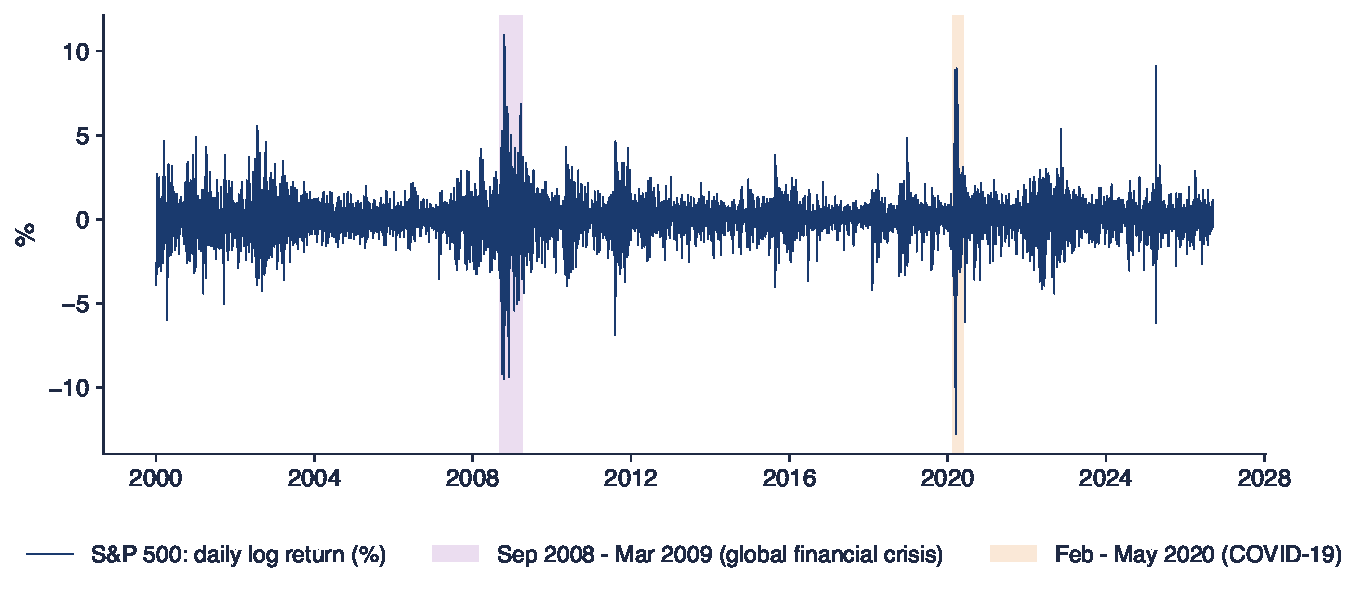
\includegraphics[width=0.97\textwidth,height=0.50\textheight,keepaspectratio]{sfm_ch9_returns.pdf}
\end{center}
\vspace{-0.25cm}
\begin{itemize}
    \item Daily log returns $r_t = 100(\ln P_t - \ln P_{t-1})$, in \%, 6\,714 days to 18 September 2026; the largest fall: $-12.8\%$ on 16 March 2020; the largest rise: $11.0\%$ on 13 October 2008
    \item Standard deviation: $0.42\%$ in 2017, $3.52\%$ from September 2008 to March 2009, $3.70\%$ from February to May 2020
    \item Large changes follow large changes, of either sign: volatility clustering \refEngle
\end{itemize}
\sfmquantlet{Ch_09}{SFM_ch9_volatility_markets}
\end{frame}

\begin{frame}{Two Storms: 2008 and 2020}
\itemsize{\footnotesize}
\begin{columns}[T]
\begin{column}{0.48\textwidth}
\centering
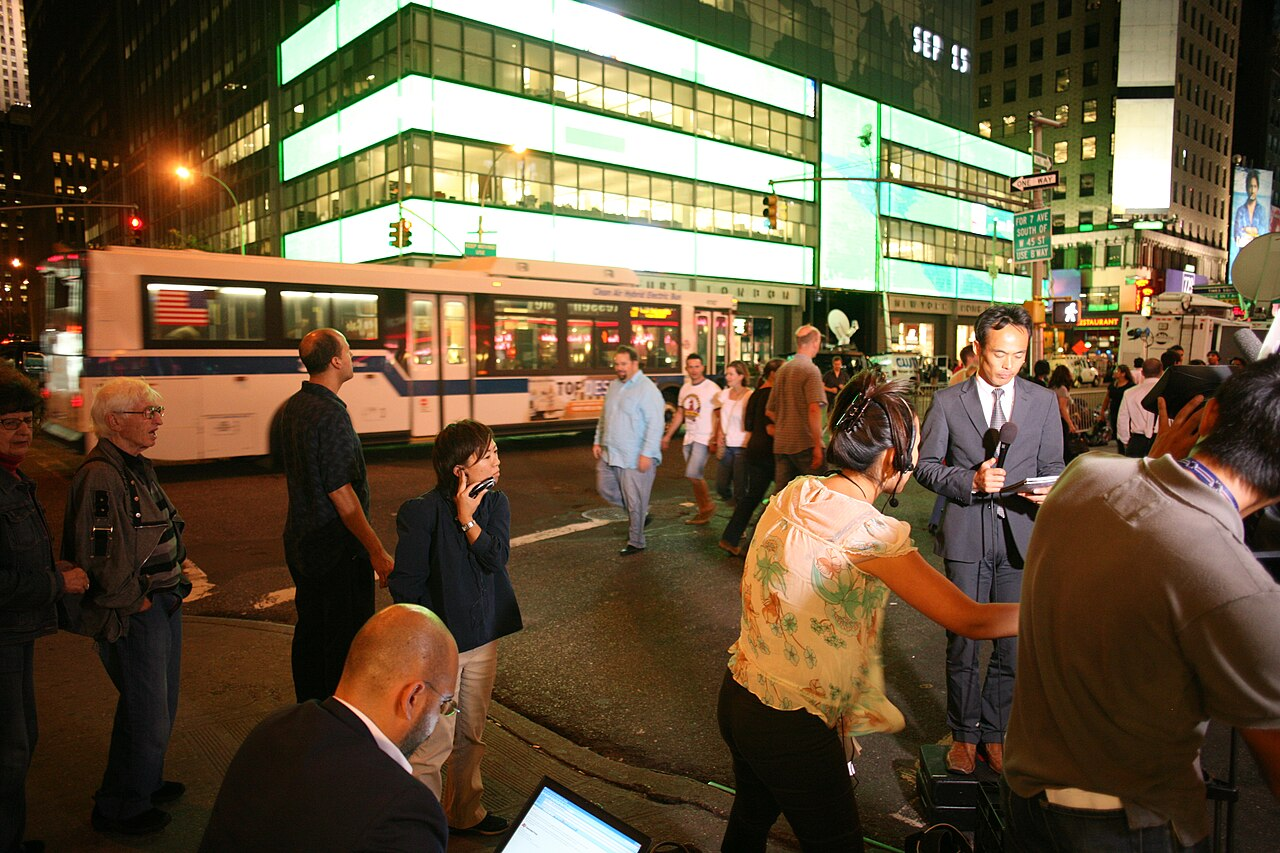
\includegraphics[height=0.30\textheight]{ch0_lehman_2008.jpg}\\[1mm]
\imgcap{Lehman Brothers headquarters, New York, 15 September 2008}
\imgcredit{https://commons.wikimedia.org/wiki/File:Lehman_Brothers-NYC-20080915.jpg}{Photo: Robert Scoble (2008); CC BY 2.0; Wikimedia Commons}
\end{column}
\begin{column}{0.48\textwidth}
\centering
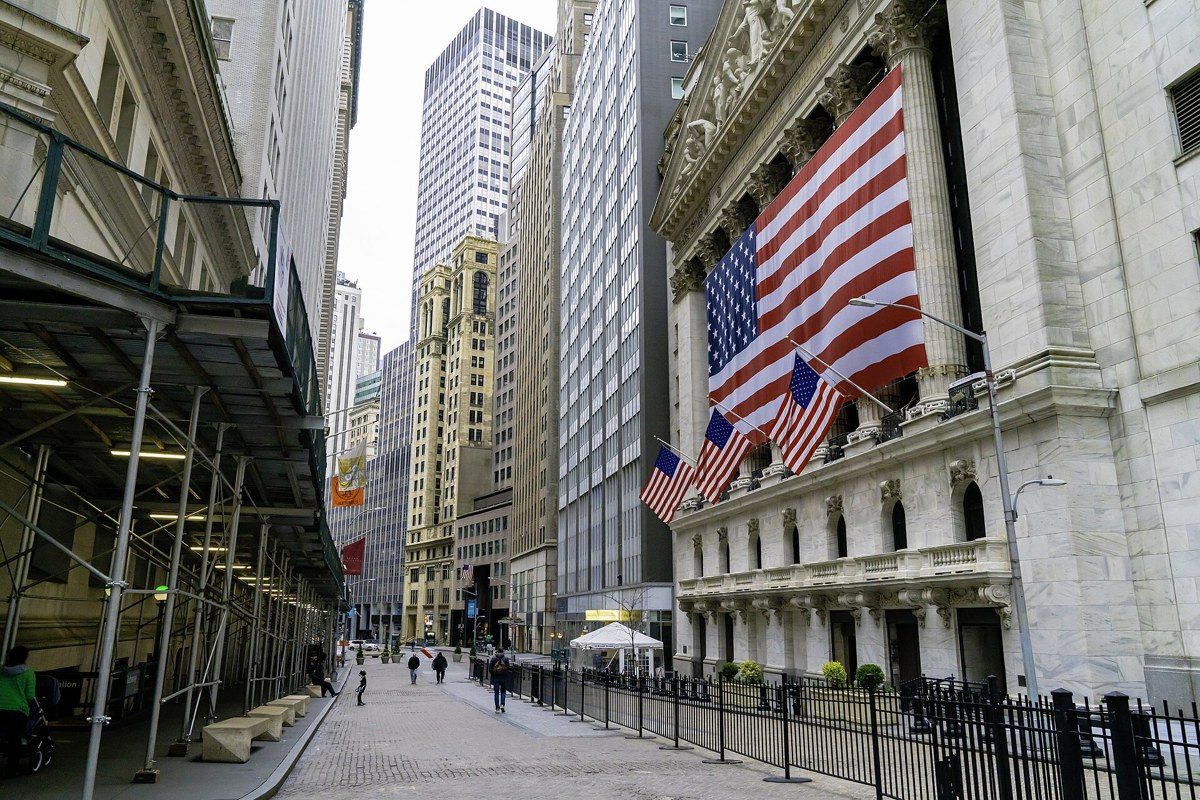
\includegraphics[height=0.30\textheight]{ch0_fidi_march_2020.jpg}\\[1mm]
\imgcap{The Financial District of New York, 25 March 2020}
\imgcredit{https://commons.wikimedia.org/wiki/File:Subdued_FiDi_(50063555551).jpg}{Photo: Billie Grace Ward (2020); CC BY 2.0; Wikimedia Commons}
\end{column}
\end{columns}\begin{itemize}
    \item 15 September 2008: Lehman Brothers files for bankruptcy; March 2020: the COVID-19 pandemic closes economies
    \item In both episodes the daily standard deviation of the S\&P 500 was 8.3 and 8.8 times that of 2017; calm returned only after months
\end{itemize}
\end{frame}

\begin{frame}{Why Model the Conditional Variance?}
\itemsize{\small}
\begin{itemize}
    \item \textbf{Risk management}: VaR (value at risk) and ES (expected shortfall) need tomorrow's volatility, not the average volatility of the last 20 years
    \begin{itemize}
        \item a constant-variance VaR is too large in calm years and too small in crises (\sfmchlink{https://danpele.github.io/SFM/EN/Courses/chapter10_var_es_backtesting.pdf}{Chapter 10})
    \end{itemize}
    \item \textbf{Portfolios}: weights depend on variances and covariances, which change over time
    \item \textbf{Derivatives}: option prices depend on the volatility expected until maturity
    \item \textbf{Inference}: tests and confidence intervals that assume a constant variance can be wrong
    \begin{itemize}
        \item this is why \sfmchlink{https://danpele.github.io/SFM/EN/Courses/chapter7_efficient_markets_random_walk_vr.pdf}{Chapter 7} needed tests that remain valid under heteroskedasticity
    \end{itemize}
\end{itemize}
\end{frame}

\begin{frame}{Stylised Facts a Volatility Model Must Reproduce}
\itemsize{\small}
\begin{itemize}
    \item \textbf{Volatility clustering}: the ACF (autocorrelation function) of $r_t^2$ is positive and decays slowly (\sfmchlink{https://danpele.github.io/SFM/EN/Courses/chapter8_volatility_estimators.pdf}{Chapter 8})
    \begin{itemize}
        \item S\&P 500: autocorrelation of $r_t^2$ at lag 1: $0.31$; at lag 50: still $0.053$
    \end{itemize}
    \item \textbf{Heavy tails}: kurtosis above 3, the value of the Normal distribution (\sfmchlink{https://danpele.github.io/SFM/EN/Courses/chapter2_classical_distributions_stylised_facts.pdf}{Chapter 2})
    \begin{itemize}
        \item S\&P 500 daily returns: kurtosis $13.7$
    \end{itemize}
    \item \textbf{Leverage effect}: falls raise volatility more than rises of the same size \refChristie
    \item \textbf{Mean reversion of volatility}: after a storm, volatility returns to a long-run level
    \item Almost no autocorrelation in $r_t$ itself (\sfmchlink{https://danpele.github.io/SFM/EN/Courses/chapter7_efficient_markets_random_walk_vr.pdf}{Chapter 7})
\end{itemize}
\end{frame}

\begin{frame}{Recap: Volatility Comes in Bursts}
\itemsize{\small}
\begin{itemize}
    \item Calm periods and storms alternate; a storm lasts for months
    \item Risk measures, portfolios, option prices and tests need the volatility of tomorrow
    \item A good model: clustering, heavy tails, leverage effect, mean reversion of volatility
\end{itemize}
\end{frame}


%=============================================================================
\section{Conditional Mean and Conditional Variance}
%=============================================================================

\begin{frame}{Conditioning on the Past}
\itemsize{\small}
\begin{itemize}
    \item $\mathcal{F}_{t-1}$: the information available at the end of day $t-1$ (past returns)
    \begin{itemize}
        \item conditional expectation $E[X \mid \mathcal{F}_{t-1}]$: the best forecast of $X$ given the past (\sfmchlink{https://danpele.github.io/SFM/EN/Courses/chapter4_probability.pdf}{Chapter 4})
    \end{itemize}
    \item \textbf{Conditional mean}: $\mu_t = E[r_t \mid \mathcal{F}_{t-1}]$
    \begin{itemize}
        \item \sfmchlink{https://danpele.github.io/SFM/EN/Courses/chapter7_efficient_markets_random_walk_vr.pdf}{Chapter 7}: for daily returns, $\mu_t$ is almost constant: $\mu_t = \mu$
    \end{itemize}
    \item \textbf{Conditional variance}: $\sigma_t^2 = \mathrm{Var}(r_t \mid \mathcal{F}_{t-1}) = E[(r_t - \mu_t)^2 \mid \mathcal{F}_{t-1}]$
    \begin{itemize}
        \item $\sigma_t$ is the \textbf{conditional volatility}: known at $t-1$, it changes from day to day
        \item \textbf{heteroskedasticity}: a variance that is not constant
    \end{itemize}
\end{itemize}
\end{frame}

\begin{frame}{The Basic Decomposition}
\itemsize{\small}
\begin{itemize}
    \item Every model of this chapter has the form $r_t = \mu + \varepsilon_t$, \quad $\varepsilon_t = \sigma_t z_t$
    \begin{itemize}
        \item $z_t$: the \textbf{innovations}, i.i.d.\ with mean 0 and variance 1 (Normal, Student-t, \dots)
        \item $\varepsilon_t$: the \textbf{shock} (the return minus its mean); $\sigma_t$ depends only on the past
    \end{itemize}
    \item Consequences
    \begin{itemize}
        \item $E[\varepsilon_t \mid \mathcal{F}_{t-1}] = \sigma_t E[z_t] = 0$: the shocks are a martingale difference, hence uncorrelated
        \item $\mathrm{Var}(\varepsilon_t \mid \mathcal{F}_{t-1}) = \sigma_t^2$: the variance is predictable
        \item the $\varepsilon_t$ are uncorrelated but not independent: $\varepsilon_t^2$ is correlated with $\varepsilon_{t-1}^2$
    \end{itemize}
    \item In the terms of \sfmchlink{https://danpele.github.io/SFM/EN/Courses/chapter7_efficient_markets_random_walk_vr.pdf}{Chapter 7}: RW1 (i.i.d. increments) is rejected, RW3 (uncorrelated increments) is kept
\end{itemize}
\end{frame}

\begin{frame}{Worked Example: Conditional and Unconditional Variance}
\itemsize{\small}
\begin{itemize}
    \item A market has calm days ($\sigma_t^2 = 0.5$) and stormy days ($\sigma_t^2 = 4.5$), each with probability $1/2$; the mean is 0
    \begin{itemize}
        \item law of total variance: $\mathrm{Var}(r_t) = E[\mathrm{Var}(r_t \mid \mathcal{F}_{t-1})] + \mathrm{Var}(E[r_t \mid \mathcal{F}_{t-1}])$
        \item step by step: $0.5 \times 0.5 + 0.5 \times 4.5 + 0 = 2.50$, so the unconditional standard deviation is $1.58\%$
    \end{itemize}
    \item The unconditional variance is an average; the conditional variance tells which day we are in
    \begin{itemize}
        \item a calm day: $\sigma_t = 0.71\%$; a stormy day: $\sigma_t = 2.12\%$; the average $1.58\%$ fits neither
    \end{itemize}
    \item A mixture of Normal distributions with different variances has heavy tails: conditional heteroskedasticity creates kurtosis
\end{itemize}
\end{frame}

\begin{frame}{Recap: Conditional Mean and Conditional Variance}
\itemsize{\small}
\begin{itemize}
    \item $r_t = \mu + \sigma_t z_t$: constant mean, conditional volatility $\sigma_t$ known one day ahead
    \item Shocks are uncorrelated but dependent through their squares
    \item Unconditional variance = average of the conditional variances
\end{itemize}
\end{frame}


%=============================================================================
\section{The ARCH Model}
%=============================================================================

\begin{frame}{1982: Robert Engle and ARCH}
\itemsize{\footnotesize}
\begin{columns}[T]
\begin{column}{0.60\textwidth}
\begin{itemize}
    \item \refEngle: \textbf{ARCH} (autoregressive conditional heteroskedasticity): today's variance depends on yesterday's squared shocks
    \begin{itemize}
        \item first application: the variance of inflation in the United Kingdom; written while Engle was visiting the London School of Economics
    \end{itemize}
    \item \href{https://www.nobelprize.org/prizes/economic-sciences/2003/summary/}{Nobel Prize 2003}: ``for methods of analyzing economic time series with time-varying volatility (ARCH)''
    \begin{itemize}
        \item shared with Clive Granger (cointegration); Nobel lecture: \refEngleN
    \end{itemize}
\end{itemize}
\end{column}
\begin{column}{0.36\textwidth}
\centering

\includegraphics[height=0.25\textheight]{ch9_engle_2022.jpg}\\[1mm]
\imgcap{Robert F. Engle (2022)}
\imgcredit{https://commons.wikimedia.org/wiki/File:0603-Kraneshares_KRBN-RobertEngle-JonDemske-16_(cropped).jpg}{Photo: Jon Demske (2022); CC BY-SA 4.0; Wikimedia Commons}\\[1mm]
\centering
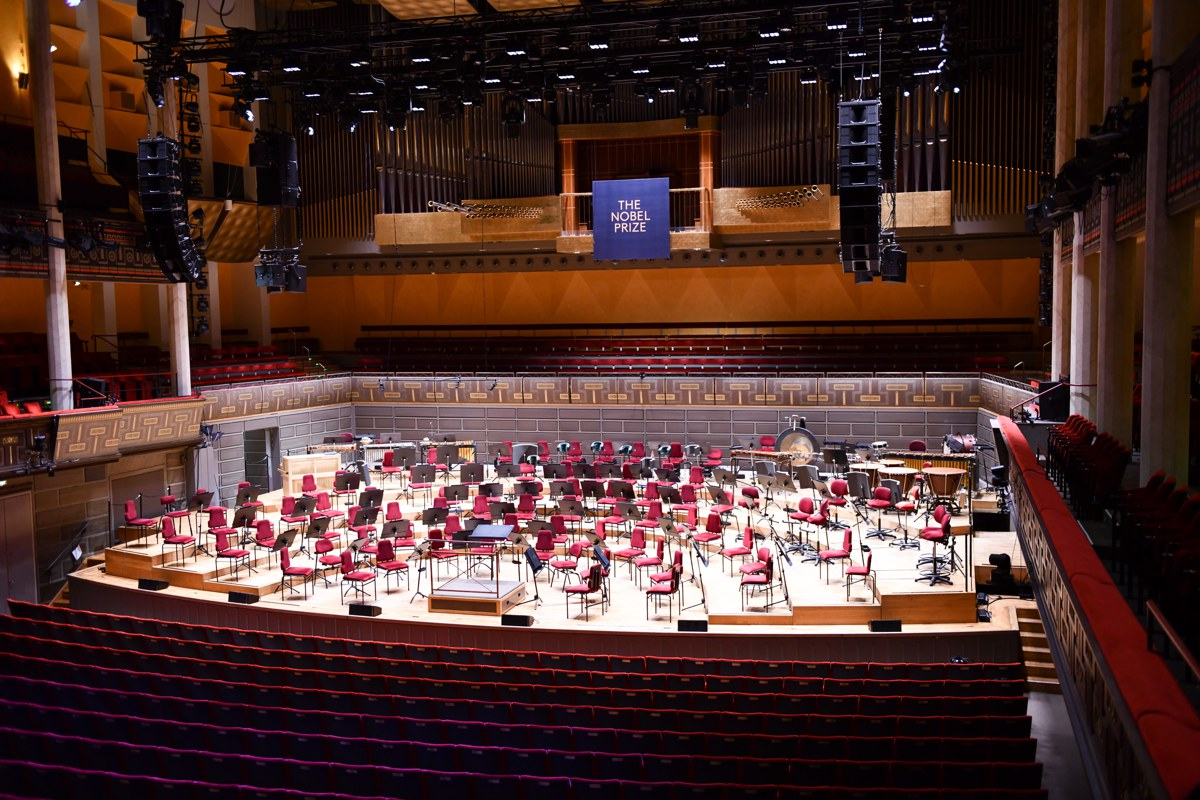
\includegraphics[height=0.16\textheight]{ch9_stockholm_concert_hall.jpg}\\[1mm]
\imgcap{Stockholm Concert Hall, venue of the Nobel Prize ceremony}
\imgcredit{https://commons.wikimedia.org/wiki/File:Konserthuset_Stockholm_(Stockholm_Concert_Hall).jpg}{Photo: Karen Zhou (2025); CC BY-SA 4.0; Wikimedia Commons}
\end{column}
\end{columns}
\end{frame}

\begin{frame}{ARCH(1): Definition}
\itemsize{\small}
\begin{itemize}
    \item $\varepsilon_t = \sigma_t z_t$, \quad $\sigma_t^2 = \omega + \alpha\,\varepsilon_{t-1}^2$, \quad $\omega > 0$, $\alpha \ge 0$
    \begin{itemize}
        \item in words: today's variance = a constant plus a share $\alpha$ of yesterday's squared shock
        \item $\omega$: the variance after a zero shock; $\alpha$: the reaction to yesterday's shock; both keep the variance positive
        \item a large shock yesterday, of either sign, raises today's variance
    \end{itemize}
    \item ``Autoregressive'': $\varepsilon_t^2$ follows an AR(1) (autoregressive) model
    \begin{itemize}
        \item write $\varepsilon_t^2 = \sigma_t^2 + v_t$ with $v_t = \sigma_t^2(z_t^2 - 1)$, $E[v_t \mid \mathcal{F}_{t-1}] = 0$
        \item then $\varepsilon_t^2 = \omega + \alpha\,\varepsilon_{t-1}^2 + v_t$: an AR(1) for the squared shocks
    \end{itemize}
    \item Hence the ACF of $\varepsilon_t^2$ is $\rho(k) = \alpha^k$ when the fourth moment exists: clustering, but a fast decay
\end{itemize}
\end{frame}

\begin{frame}{ARCH(1): Properties}
\itemsize{\small}
\begin{itemize}
    \item Mean and autocorrelation: $E[\varepsilon_t] = 0$, $\mathrm{Cov}(\varepsilon_t, \varepsilon_{t-k}) = 0$ for $k \ne 0$
    \item \textbf{Unconditional variance} (if $\alpha < 1$): take expectations in $\sigma_t^2 = \omega + \alpha\varepsilon_{t-1}^2$
    \begin{itemize}
        \item $\bar\sigma^2 = E[\varepsilon_t^2] = \omega + \alpha\bar\sigma^2$, so $\bar\sigma^2 = \omega/(1 - \alpha)$
    \end{itemize}
    \item \textbf{Kurtosis} with Normal $z_t$ (if $3\alpha^2 < 1$): $K = \dfrac{E[\varepsilon_t^4]}{(E[\varepsilon_t^2])^2} = 3\,\dfrac{1 - \alpha^2}{1 - 3\alpha^2} > 3$
    \begin{itemize}
        \item Normal innovations, but heavy-tailed returns \refFHH
        \item if $\alpha \ge 1/\sqrt{3} = 0.577$, the fourth moment is infinite
    \end{itemize}
    \item \textbf{Worked example}: $\omega = 0.5$, $\alpha = 0.5$
    \begin{itemize}
        \item $\bar\sigma^2 = 0.5/0.5 = 1.00$; $K = 3 \times 0.75/0.25 = 9.0$; after a shock $\varepsilon_{t-1} = 2$: $\sigma_t^2 = 0.5 + 0.5 \times 4 = 2.50$, $\sigma_t = 1.58$
    \end{itemize}
\end{itemize}
\end{frame}

\begin{frame}{Simulated Paths: i.i.d., ARCH(1) and GARCH(1,1)}
\itemsize{\footnotesize}
\begin{center}
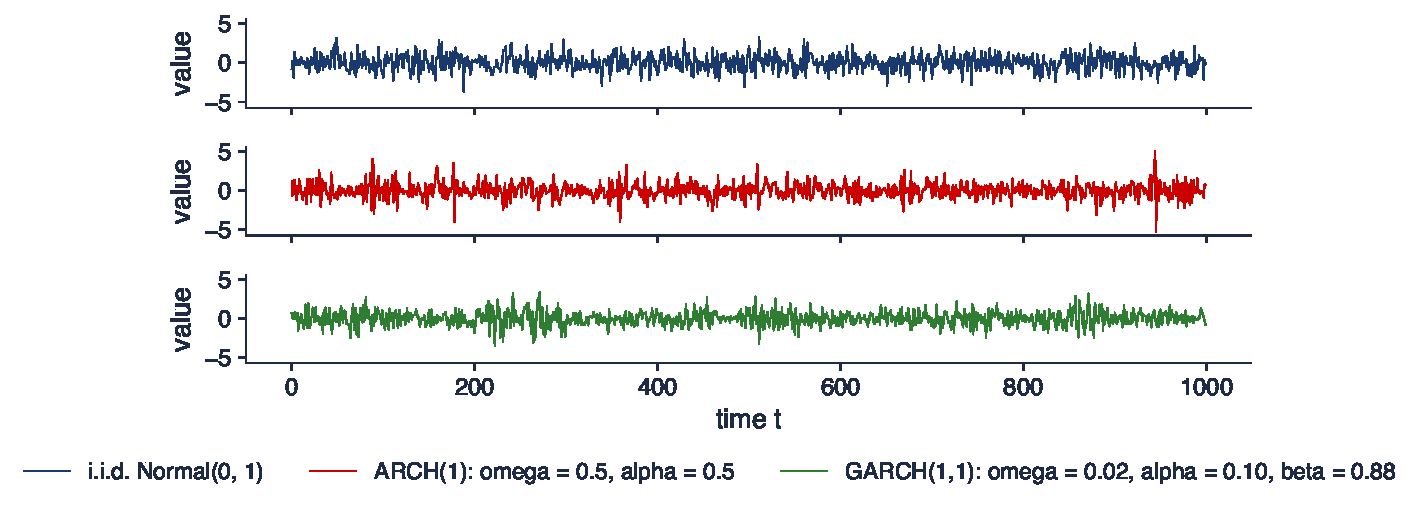
\includegraphics[width=0.97\textwidth,height=0.48\textheight,keepaspectratio]{sfm_ch9_simulated.pdf}
\end{center}
\vspace{-0.25cm}
\begin{itemize}
    \item Three series of 1000 values with unconditional variance 1; ARCH(1) with $\omega = \alpha = 0.5$, GARCH(1,1) with $\omega = 0.02$, $\alpha = 0.10$, $\beta = 0.88$ (next section)
    \item Sample kurtosis: i.i.d.\ $3.12$, ARCH $4.91$, GARCH $3.74$; theory: 3, $9.0$, $6.06$; the fourth moment converges slowly
    \item ARCH(1) gives isolated spikes; GARCH(1,1) gives long calm and long agitated periods, as in real returns
\end{itemize}
\sfmquantlet{Ch_09}{SFM_ch9_simulation_likelihood}
\end{frame}

\begin{frame}{ARCH($q$) and Its Limits}
\itemsize{\footnotesize}
\begin{itemize}
    \item \textbf{ARCH($q$)}: $\sigma_t^2 = \omega + \alpha_1\varepsilon_{t-1}^2 + \dots + \alpha_q\varepsilon_{t-q}^2$, $\alpha_i \ge 0$; stationary if $\sum_i \alpha_i < 1$
    \begin{itemize}
        \item $q$: the number of lags; $\alpha_i$: the reaction to the shock of $i$ days ago
        \item the effect of a shock lasts exactly $q$ days; real clustering lasts for months
    \end{itemize}
    \item Testing for ARCH effects: the ARCH-LM test of Engle (regression of $\hat\varepsilon_t^2$ on its lags), \sfmchlink{https://danpele.github.io/SFM/EN/Courses/chapter8_volatility_estimators.pdf}{Chapter 8}
\end{itemize}\begin{center}
\footnotesize
\begin{tabular}{lrrrrr}
\toprule
S\&P 500, Normal $z_t$ & parameters & log-likelihood & AIC & BIC & $\sum\alpha_i$ (+$\beta$) \\
\midrule
ARCH(1) & 3 & $-10305.5$ & 20617.0 & 20637.5 & $0.394$ \\
ARCH(5) & 7 & $-9340.5$ & 18695.1 & 18742.7 & $0.816$ \\
ARCH(10) & 12 & $-9227.6$ & 18479.3 & 18561.0 & $0.849$ \\
GARCH(1,1) & 4 & $-9218.0$ & \textbf{18444.0} & \textbf{18471.2} & $0.980$ \\
\bottomrule
\end{tabular}
\end{center}
\begin{itemize}
    \item Interpretation: ARCH needs ten lags and still loses to GARCH(1,1), which has four parameters (AIC and BIC: smaller is better, Section 10)
\end{itemize}\sfmquantlet{Ch_09}{SFM_ch9_garch_estimation}
\end{frame}

\begin{frame}{Recap: The ARCH Model}
\itemsize{\small}
\begin{itemize}
    \item $\sigma_t^2 = \omega + \sum_i\alpha_i\varepsilon_{t-i}^2$: an AR model for the squared shocks
    \item Unconditional variance $\omega/(1 - \sum\alpha_i)$; kurtosis above 3 even with Normal innovations
    \item Real clustering needs many lags: the motivation for GARCH
\end{itemize}
\end{frame}


%=============================================================================
\section{The GARCH(1,1) Model}
%=============================================================================

\begin{frame}{1986: Tim Bollerslev and GARCH}
\itemsize{\small}
\begin{columns}[T]
\begin{column}{0.56\textwidth}
\begin{itemize}
    \item \refBoll, a doctoral student of Engle at the University of California, San Diego: add yesterday's variance to the equation
    \begin{itemize}
        \item \textbf{GARCH} (generalised ARCH): a few parameters replace a long ARCH($q$)
    \end{itemize}
    \item Student-t innovations for returns: \refBollT
    \item GARCH(1,1) is still the benchmark: \refHL{} compared 330 models and found it hard to beat on exchange rates
\end{itemize}
\end{column}
\begin{column}{0.40\textwidth}
\centering
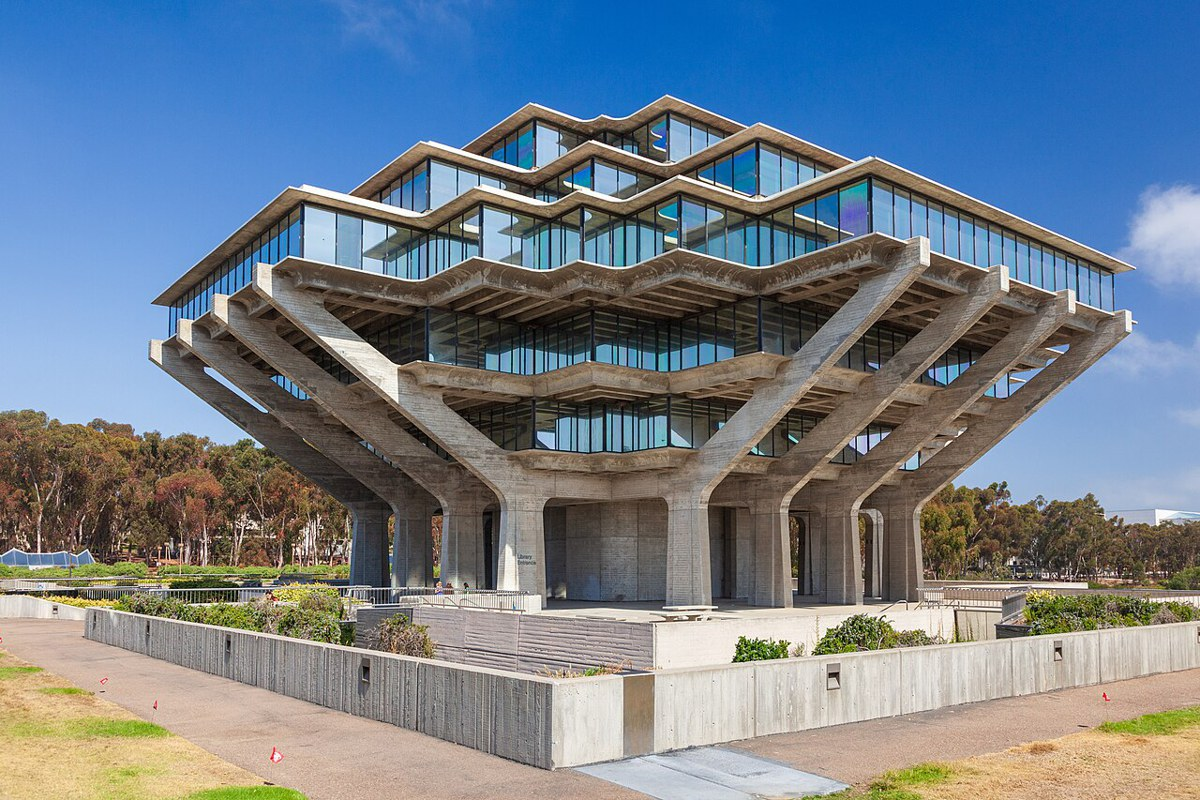
\includegraphics[height=0.36\textheight]{ch9_ucsd_geisel_2010.jpg}\\[1mm]
\imgcap{Geisel Library, University of California, San Diego}
\imgcredit{https://commons.wikimedia.org/wiki/File:Geisel_Library,_UC_San_Diego.jpg}{Photo: Stephen Bay (2010); CC BY 4.0; Wikimedia Commons}
\end{column}
\end{columns}
\end{frame}

\begin{frame}{GARCH(1,1): Definition}
\itemsize{\small}
\begin{itemize}
    \item $r_t = \mu + \varepsilon_t$, \quad $\varepsilon_t = \sigma_t z_t$, \quad $\sigma_t^2 = \omega + \alpha\,\varepsilon_{t-1}^2 + \beta\,\sigma_{t-1}^2$
    \begin{itemize}
        \item $\omega > 0$, $\alpha \ge 0$, $\beta \ge 0$: the variance stays positive
    \end{itemize}
    \item Reading the parameters
    \begin{itemize}
        \item $\alpha$: the \textbf{reaction} to yesterday's news (size of the jump after a shock)
        \item $\beta$: the \textbf{memory} of the variance (how much of yesterday's level is kept)
        \item $\alpha + \beta$: the \textbf{persistence}; $\omega$ sets the long-run level
    \end{itemize}
    \item By recursion, an ARCH($\infty$) with geometric weights
    \begin{itemize}
        \item $\sigma_t^2 = \dfrac{\omega}{1 - \beta} + \alpha\sum_{j=0}^{\infty}\beta^j\,\varepsilon_{t-1-j}^2$: all past shocks matter, with decaying weights
        \item the shock of $j + 1$ days ago gets the weight $\alpha\beta^j$
    \end{itemize}
\end{itemize}
\end{frame}

\begin{frame}{Stationarity, Long-Run Variance and Kurtosis}
\itemsize{\small}
\begin{itemize}
    \item As for ARCH: $\varepsilon_t^2 = \omega + (\alpha + \beta)\varepsilon_{t-1}^2 + v_t - \beta v_{t-1}$, an ARMA(1,1) for the squared shocks
    \begin{itemize}
        \item $v_t = \varepsilon_t^2 - \sigma_t^2$: the surprise in the squared shock, as for ARCH(1)
        \item ARMA: autoregressive moving average; the ACF of $\varepsilon_t^2$ decays like $(\alpha + \beta)^k$ at lag $k$
    \end{itemize}
    \item \textbf{Covariance stationary} if $\alpha + \beta < 1$; then the \textbf{unconditional (long-run) variance} is
    \begin{itemize}
        \item $\bar\sigma^2 = E[\sigma_t^2] = \dfrac{\omega}{1 - \alpha - \beta}$, \quad annualised volatility $\sqrt{252\,\bar\sigma^2}$ for 252 trading days
    \end{itemize}
    \item Kurtosis with Normal $z_t$, if $(\alpha + \beta)^2 + 2\alpha^2 < 1$: $K = 3\,\dfrac{1 - (\alpha + \beta)^2}{1 - (\alpha + \beta)^2 - 2\alpha^2} > 3$
    \begin{itemize}
        \item $\alpha = 0.10$, $\beta = 0.88$: $(\alpha + \beta)^2 + 2\alpha^2 = 0.9804$, $K = 6.06$
    \end{itemize}
\end{itemize}
\end{frame}

\begin{frame}{Persistence and Half-Life}
\itemsize{\small}
\begin{itemize}
    \item Forecast of the variance $h$ days ahead (derived in Section 11): $E[\sigma_{t+h}^2 \mid \mathcal{F}_t] - \bar\sigma^2 = (\alpha + \beta)^{h-1}(\sigma_{t+1}^2 - \bar\sigma^2)$
    \begin{itemize}
        \item $E[\cdot \mid \mathcal{F}_t]$: the forecast made at the end of day $t$; $\bar\sigma^2$: the long-run variance
        \item a deviation from the long-run variance shrinks by the factor $\alpha + \beta$ each day
    \end{itemize}
    \item \textbf{Half-life}: the number of days after which half of a variance shock is gone
    \begin{itemize}
        \item $(\alpha + \beta)^{h} = 1/2 \;\Rightarrow\; h_{1/2} = \dfrac{\ln 0.5}{\ln(\alpha + \beta)}$
        \item $\alpha + \beta = 0.90$: 6.6 days; $0.98$: 34.3 days; $0.99$: 69.0 days: small changes near 1 matter a lot
    \end{itemize}
    \item Daily equity returns: $\alpha$ around 0.05--0.15, $\beta$ around 0.80--0.93, $\alpha + \beta$ close to 1 (Section 7)
\end{itemize}
\end{frame}

\begin{frame}{Worked Example: One GARCH(1,1) Step}
\itemsize{\small}
\begin{itemize}
    \item Daily returns in \%: $\omega = 0.02$, $\alpha = 0.10$, $\beta = 0.88$, $\mu = 0$
    \item Long-run quantities
    \begin{itemize}
        \item persistence $\alpha + \beta = 0.98$; $\bar\sigma^2 = 0.02/(1 - 0.98) = 1.00$; annualised volatility $\sqrt{252 \times 1.00} = 15.9\%$
        \item half-life $\ln 0.5/\ln 0.98 = 34.3$ days
    \end{itemize}
    \item Today: $\sigma_t^2 = 1.2$ and the return is $r_t = -3\%$
    \begin{itemize}
        \item tomorrow: $\sigma_{t+1}^2 = 0.02 + 0.10 \times 9 + 0.88 \times 1.2 = 1.976$, $\sigma_{t+1} = 1.41\%$
        \item the shock raised the variance from 1.2 to almost 2; it then decays towards 1.00 with the factor 0.98 per day
    \end{itemize}
\end{itemize}
\end{frame}

\begin{frame}{IGARCH and the EWMA Link}
\itemsize{\small}
\begin{itemize}
    \item \textbf{IGARCH} (integrated GARCH) \refEB: $\alpha + \beta = 1$
    \begin{itemize}
        \item shocks to the variance never die out: no half-life, no finite unconditional variance
        \item the forecast of the variance is the same for every horizon
    \end{itemize}
    \item \textbf{EWMA} (exponentially weighted moving average, \sfmchlink{https://danpele.github.io/SFM/EN/Courses/chapter8_volatility_estimators.pdf}{Chapter 8}): $\sigma_t^2 = \lambda\sigma_{t-1}^2 + (1 - \lambda)r_{t-1}^2$
    \begin{itemize}
        \item this is IGARCH with $\omega = 0$, $\alpha = 1 - \lambda$, $\beta = \lambda$; RiskMetrics uses $\lambda = 0.94$ for daily data
        \item EWMA: nothing to estimate, but no mean reversion; GARCH: three parameters, and volatility returns to $\bar\sigma$
    \end{itemize}
    \item \textbf{Question for the room}: an analyst forecasts the volatility one year ahead with EWMA right after a crash. What goes wrong?
    \begin{itemize}
        \item \textbf{Answer}: EWMA keeps today's crisis level for the whole year; GARCH lets it decay towards the long-run level
    \end{itemize}
\end{itemize}
\end{frame}

\begin{frame}{Recap: The GARCH(1,1) Model}
\itemsize{\small}
\begin{itemize}
    \item $\sigma_t^2 = \omega + \alpha\varepsilon_{t-1}^2 + \beta\sigma_{t-1}^2$: reaction $\alpha$, memory $\beta$
    \item $\alpha + \beta < 1$: long-run variance $\omega/(1 - \alpha - \beta)$, half-life $\ln 0.5/\ln(\alpha + \beta)$
    \item $\alpha + \beta = 1$: IGARCH; EWMA is an IGARCH without $\omega$
\end{itemize}
\end{frame}


%=============================================================================
\section{Estimation by Maximum Likelihood}
%=============================================================================

\begin{frame}{The Likelihood of a GARCH Model}
\itemsize{\small}
\begin{itemize}
    \item The returns are dependent, so we factor the joint density into conditional densities
    \begin{itemize}
        \item $f$: a probability density; $T$: the number of returns; $\theta$: the vector of parameters; $\ell$: the log-likelihood
        \item $f(r_1, \dots, r_T) = f(r_1)\prod_{t=2}^{T} f(r_t \mid \mathcal{F}_{t-1})$, and $r_t \mid \mathcal{F}_{t-1} \sim N(\mu, \sigma_t^2)$ for Normal innovations
    \end{itemize}
    \item \textbf{Conditional log-likelihood} with $\theta = (\mu, \omega, \alpha, \beta)$:
    \begin{itemize}
        \item $\ell(\theta) = -\dfrac12\sum_{t=2}^{T}\Big[\ln(2\pi) + \ln\sigma_t^2(\theta) + \dfrac{(r_t - \mu)^2}{\sigma_t^2(\theta)}\Big]$
        \item in words: each day adds a penalty for a large $\sigma_t^2$ and a penalty for a squared error that is large relative to $\sigma_t^2$
        \item $\sigma_t^2(\theta)$ is computed recursively from a starting value $\sigma_1^2$ (for example the sample variance)
    \end{itemize}
    \item \textbf{MLE} (maximum likelihood estimation): $\hat\theta = \arg\max_\theta \ell(\theta)$, under $\omega > 0$, $\alpha, \beta \ge 0$, $\alpha + \beta < 1$
    \begin{itemize}
        \item no closed form: a numerical optimiser searches for the maximum \refFHH
    \end{itemize}
\end{itemize}
\end{frame}

\begin{frame}{The Likelihood of ARCH(1)}
\itemsize{\footnotesize}
\begin{center}
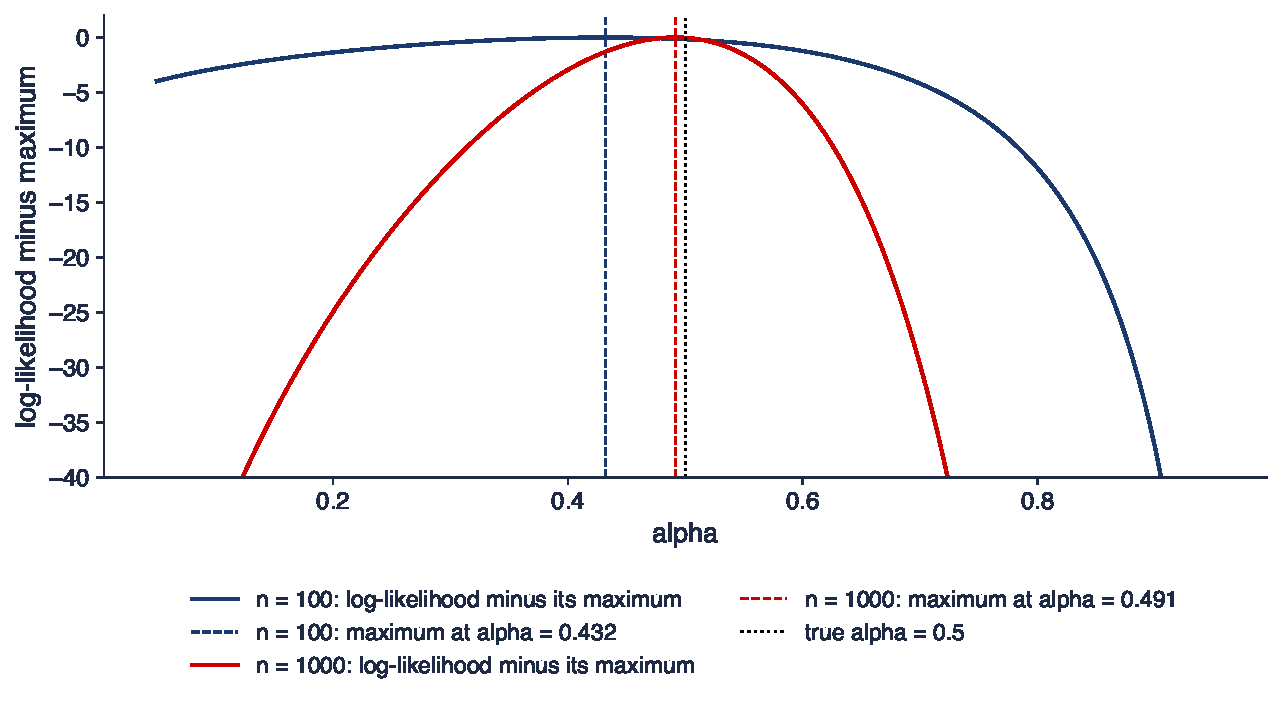
\includegraphics[width=0.97\textwidth,height=0.50\textheight,keepaspectratio]{sfm_ch9_lik_arch1.pdf}
\end{center}
\vspace{-0.25cm}
\begin{itemize}
    \item Simulated ARCH(1) with $\omega = \alpha = 0.5$; $\ell(\alpha)$ with $\omega = 1 - \alpha$, as in SFElikarch1; each curve minus its maximum
    \item $n = 100$: $\hat\alpha = 0.432$ (standard error $0.127$); $n = 1000$: $\hat\alpha = 0.491$ ($0.035$)
    \item Interpretation: more data make the curve sharper; its curvature at the maximum gives the standard error
\end{itemize}
\sfmquantlet{Ch_09}{SFM_ch9_simulation_likelihood}
\end{frame}

\begin{frame}{The Likelihood of GARCH(1,1)}
\itemsize{\footnotesize}
\begin{center}
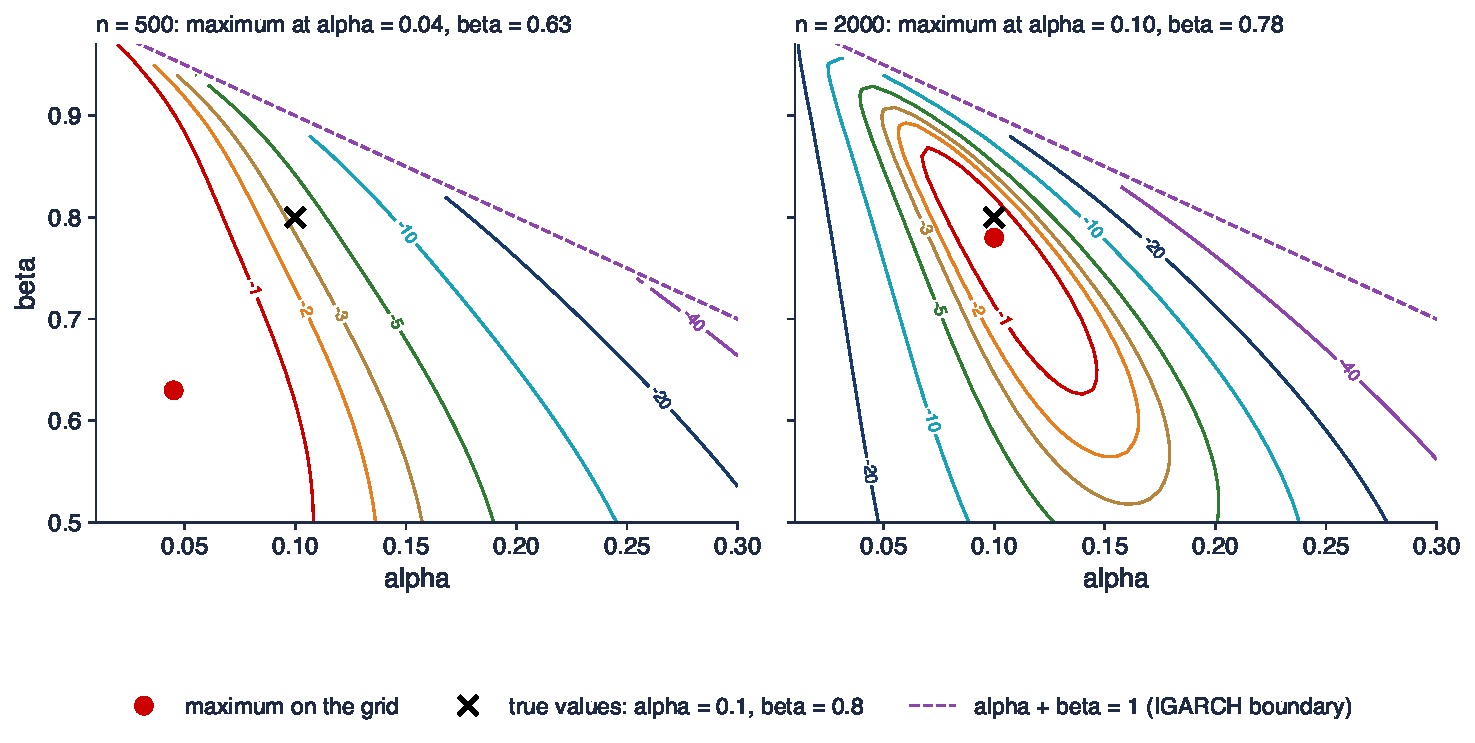
\includegraphics[width=0.97\textwidth,height=0.48\textheight,keepaspectratio]{sfm_ch9_lik_garch.pdf}
\end{center}
\vspace{-0.25cm}
\begin{itemize}
    \item Simulated GARCH(1,1), $\omega = 0.1$, $\alpha = 0.1$, $\beta = 0.8$; $\omega$ set so that the unconditional variance equals the sample variance, as in SFElikgarch; contours: log-likelihood minus its maximum
    \item $n = 500$: maximum at $(0.04, 0.63)$, far from the truth; $n = 2000$: $(0.10, 0.78)$
    \item Interpretation: a long, flat ridge along which $\alpha$ and $\beta$ trade off: GARCH needs long samples
\end{itemize}
\sfmquantlet{Ch_09}{SFM_ch9_simulation_likelihood}
\end{frame}

\begin{frame}{Estimation Step by Step and with a Package}
\itemsize{\footnotesize}
\begin{center}
\footnotesize
\begin{tabular}{lrrrr}
\toprule
S\&P 500, GARCH(1,1)-N & step by step (SE) & \texttt{arch} & classic SE & robust SE \\
\midrule
$\mu$ & $0.0614$ ($0.0098$) & $0.0615$ & $0.0098$ & $0.0100$ \\
$\omega$ & $0.0253$ ($0.0030$) & $0.0254$ & $0.0030$ & $0.0048$ \\
$\alpha$ & $0.1205$ ($0.0086$) & $0.1206$ & $0.0086$ & $0.0118$ \\
$\beta$ & $0.8600$ ($0.0091$) & $0.8599$ & $0.0091$ & $0.0125$ \\
\bottomrule
\end{tabular}
\end{center}
\begin{itemize}
    \item Step by step: write $-\ell(\theta)$ in Python and minimise it with \texttt{scipy.optimize.minimize} under $\alpha + \beta < 1$
    \begin{itemize}
        \item the two routes differ only in the start-up of $\sigma_t^2$ and in the optimiser; log-likelihood $-9219.9$ against $-9218.0$
    \end{itemize}
    \item SE (standard error), classic: from the inverse Hessian (the curvature of $\ell$); robust: valid when $z_t$ is not Normal \refBW
    \item Interpretation: the robust SE are about 1.4 times larger (1.6 for $\omega$): with heavy-tailed $z_t$ the classic SE overstate the precision
\end{itemize}\sfmquantlet{Ch_09}{SFM_ch9_garch_estimation}
\end{frame}

\begin{frame}{Quasi-Maximum Likelihood}
\itemsize{\small}
\begin{itemize}
    \item \textbf{QMLE} (quasi-maximum likelihood estimation): maximise the Normal likelihood even if $z_t$ is not Normal
    \begin{itemize}
        \item the estimates are still consistent if $\mu$ and $\sigma_t^2$ are correctly specified \refBW
        \item but the classic SE are wrong: use the robust (``sandwich'') SE
    \end{itemize}
    \item Practical rules
    \begin{itemize}
        \item report robust SE (the default of \texttt{arch})
        \item use at least 1000--2000 daily observations; returns in \% avoid numerical problems with tiny $\omega$
        \item an estimate on the boundary ($\alpha + \beta = 1$) has no usual standard error: report it as IGARCH
    \end{itemize}
    \item A better innovation distribution gives more efficient estimates: next section
\end{itemize}
\end{frame}

\begin{frame}{Recap: Estimation by Maximum Likelihood}
\itemsize{\small}
\begin{itemize}
    \item $\ell(\theta)$ = sum of conditional log-densities; $\sigma_t^2(\theta)$ computed recursively
    \item The likelihood surface has a ridge in $(\alpha, \beta)$: long samples needed
    \item Report robust (Bollerslev--Wooldridge) standard errors
\end{itemize}
\end{frame}


%=============================================================================
\section{Heavy-Tailed Innovations}
%=============================================================================

\begin{frame}{Student-t and Skewed-t Innovations}
\itemsize{\small}
\begin{itemize}
    \item GARCH with Normal $z_t$ explains only part of the kurtosis: S\&P 500 returns $13.7$, standardised residuals $\hat z_t = \hat\varepsilon_t/\hat\sigma_t$: $4.7$
    \begin{itemize}
        \item the remaining heavy tails must come from the distribution of $z_t$
    \end{itemize}
    \item \textbf{Standardised Student-t} with $\nu > 2$ degrees of freedom (\sfmchlink{https://danpele.github.io/SFM/EN/Courses/chapter2_classical_distributions_stylised_facts.pdf}{Chapter 2}) \refBollT
    \begin{itemize}
        \item $t_\nu$: a Student-t variable with $\nu$ degrees of freedom; $z_t = t_\nu\sqrt{(\nu - 2)/\nu}$ has variance 1
        \item a small $\nu$ means heavy tails: kurtosis $3 + 6/(\nu - 4)$ for $\nu > 4$; $\nu \to \infty$: the Normal distribution
        \item $\nu$ is estimated together with $(\mu, \omega, \alpha, \beta)$
    \end{itemize}
    \item \textbf{Skewed t} \refHansen: one more parameter $\lambda \in (-1, 1)$; $\lambda < 0$: a longer left tail
    \begin{itemize}
        \item nested models: Normal $\subset$ t $\subset$ skewed t; compare them with likelihood-ratio tests or AIC/BIC (\sfmchlink{https://danpele.github.io/SFM/EN/Courses/chapter6_model_selection_risk_management.pdf}{Chapter 6})
    \end{itemize}
\end{itemize}
\end{frame}

\begin{frame}{S\&P 500: Three Innovation Distributions}
\itemsize{\footnotesize}
\begin{center}
\footnotesize
\begin{tabular}{lrrrrrrr}
\toprule
GARCH(1,1) & $\omega$ & $\alpha$ & $\beta$ & $\nu$ & $\lambda$ & log-lik. & $\alpha + \beta$ \\
\midrule
Normal & $0.0254$ & $0.121$ & $0.860$ & -- & -- & $-9218.0$ & $0.980$ \\
Student-t & $0.0157$ & $0.123$ & $0.872$ & $6.26$ & -- & $-9062.5$ & $0.995$ \\
skewed t & $0.0153$ & $0.120$ & $0.872$ & $6.92$ & $-0.114$ & $-9038.4$ & $0.993$ \\
\bottomrule
\end{tabular}
\end{center}
\begin{itemize}
    \item Likelihood-ratio statistic $2(\ell_1 - \ell_0)$ ($\ell_1$, $\ell_0$: maximised log-likelihoods of the larger and the smaller model): t against Normal $311.0$ (1 restriction, $\chi^2_{0.95}(1) = 3.84$); skewed t against t $48.1$: both reject the smaller model
    \item $\hat\nu = 6.26$: tails far heavier than Normal; $\hat\lambda = -0.114$: large falls more frequent than large rises
    \item Interpretation: $\alpha$ and $\beta$ hardly change; the innovation distribution matters for tail quantiles (VaR), less for $\sigma_t$
\end{itemize}\sfmquantlet{Ch_09}{SFM_ch9_garch_estimation}
\end{frame}

\begin{frame}{QQ Plots of the Standardised Residuals}
\itemsize{\footnotesize}
\begin{center}
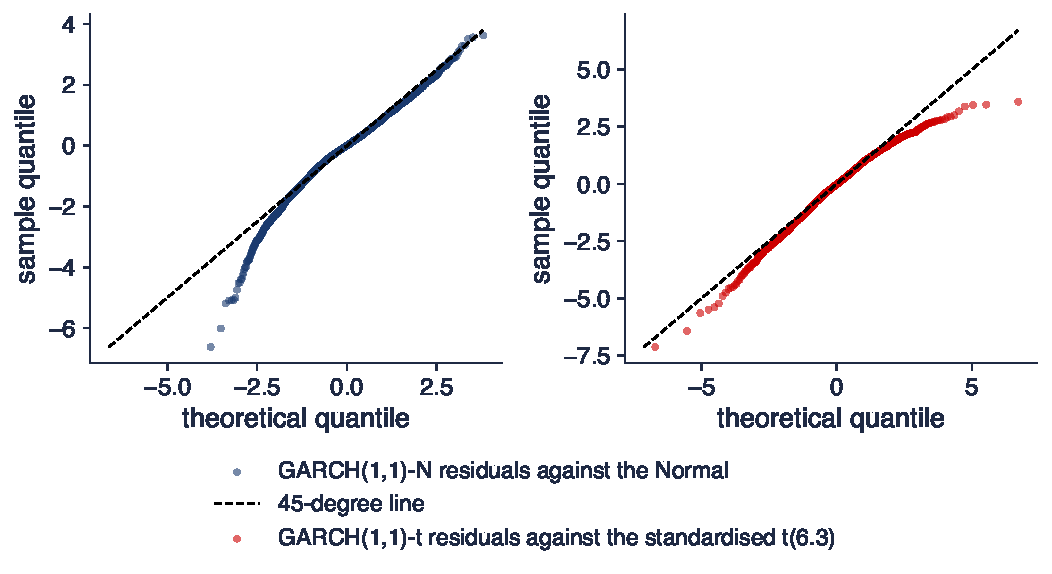
\includegraphics[width=0.97\textwidth,height=0.50\textheight,keepaspectratio]{sfm_ch9_qq.pdf}
\end{center}
\vspace{-0.25cm}
\begin{itemize}
    \item Left: residuals of the Normal GARCH against the Normal distribution: the 0.1\% quantile is $-4.81$, against $-3.09$ in theory
    \item Right: residuals of GARCH-t against the standardised t with $\hat\nu = 6.3$: $-4.79$ against $-4.19$: much closer; the largest falls are still deeper
    \item Interpretation: the left tail is the problem: a reason for skewed innovations and for asymmetric models (Section 8)
\end{itemize}
\sfmquantlet{Ch_09}{SFM_ch9_garch_estimation}
\end{frame}

\begin{frame}{Recap: Heavy-Tailed Innovations}
\itemsize{\small}
\begin{itemize}
    \item GARCH explains part of the kurtosis; the rest comes from $z_t$
    \item Student-t ($\nu$) and skewed t ($\nu$, $\lambda$) improve the likelihood strongly
    \item The distribution of $z_t$ decides the VaR quantile
\end{itemize}
\end{frame}


%=============================================================================
\section{GARCH in Six Markets}
%=============================================================================

\begin{frame}{GARCH(1,1)-t Estimates}
\itemsize{\footnotesize}
\begin{center}
\scriptsize
\begin{tabular}{lrrrrrrrr}
\toprule
& from & $\alpha$ & $\beta$ & $\nu$ & $\alpha + \beta$ & half-life & long-run vol. & sample vol. \\
\midrule
S\&P 500 & 2000 & $0.123$ & $0.872$ & $6.26$ & $0.995$ & 131 & 27.3 & 19.2 \\
DAX & 2000 & $0.097$ & $0.895$ & $7.08$ & $0.992$ & 88 & 25.9 & 22.4 \\
BET & 2000 & $0.192$ & $0.799$ & $5.01$ & $0.991$ & 74 & 34.7 & 22.1 \\
Bitcoin & 2014 & $0.109$ & $0.891$ & $3.18$ & $1.000$ & -- & -- & 66.6 \\
TLV & 2010 & $0.139$ & $0.824$ & $4.91$ & $0.963$ & 18 & 28.2 & 26.5 \\
SNP & 2010 & $0.135$ & $0.807$ & $4.81$ & $0.942$ & 12 & 25.6 & 24.5 \\
\bottomrule
\end{tabular}
\end{center}
\begin{itemize}
    \item Daily log returns in \% to 18 September 2026; robust SE of $\hat\alpha$ and $\hat\beta$ between 0.010 and 0.041; half-life in days; volatilities annualised with the actual number of observations per year, in \%
    \item Indices: $\alpha + \beta$ between 0.991 and 0.995, half-lives of 74--131 trading days; BVB stocks: shorter memory (TLV 18 days, SNP 12 days)
    \item BET: the largest $\alpha$ (0.192): a stronger reaction to news; all $\hat\nu$ between 3.2 and 7.1: heavy tails everywhere
\end{itemize}\sfmquantlet{Ch_09}{SFM_ch9_volatility_markets}
\end{frame}

\begin{frame}{Interpretation: Bitcoin and the Long-Run Volatility}
\itemsize{\small}
\begin{itemize}
    \item Bitcoin: $\hat\alpha + \hat\beta = 1.0000$, on the boundary $\alpha + \beta < 1$: an IGARCH
    \begin{itemize}
        \item no half-life and no long-run volatility: the model behaves like an EWMA with $\lambda \approx 0.891$
        \item $\hat\nu = 3.18$: extremely heavy tails (the fourth moment of $z_t$ does not exist)
    \end{itemize}
    \item \textbf{Question for the room}: S\&P 500: long-run volatility 27.3\%, sample volatility 19.2\%. Is the model wrong?
    \begin{itemize}
        \item \textbf{Answer}: not necessarily: $\bar\sigma^2 = \omega/(1 - \alpha - \beta)$ divides by $1 - \alpha - \beta = 0.0053$, a small and imprecise number
        \item the Normal GARCH gives 18.1\%; the long-run level is the least reliable output of a persistent GARCH
    \end{itemize}
\end{itemize}
\end{frame}

\begin{frame}{Conditional Volatility: S\&P 500 and DAX}
\itemsize{\footnotesize}
\begin{center}
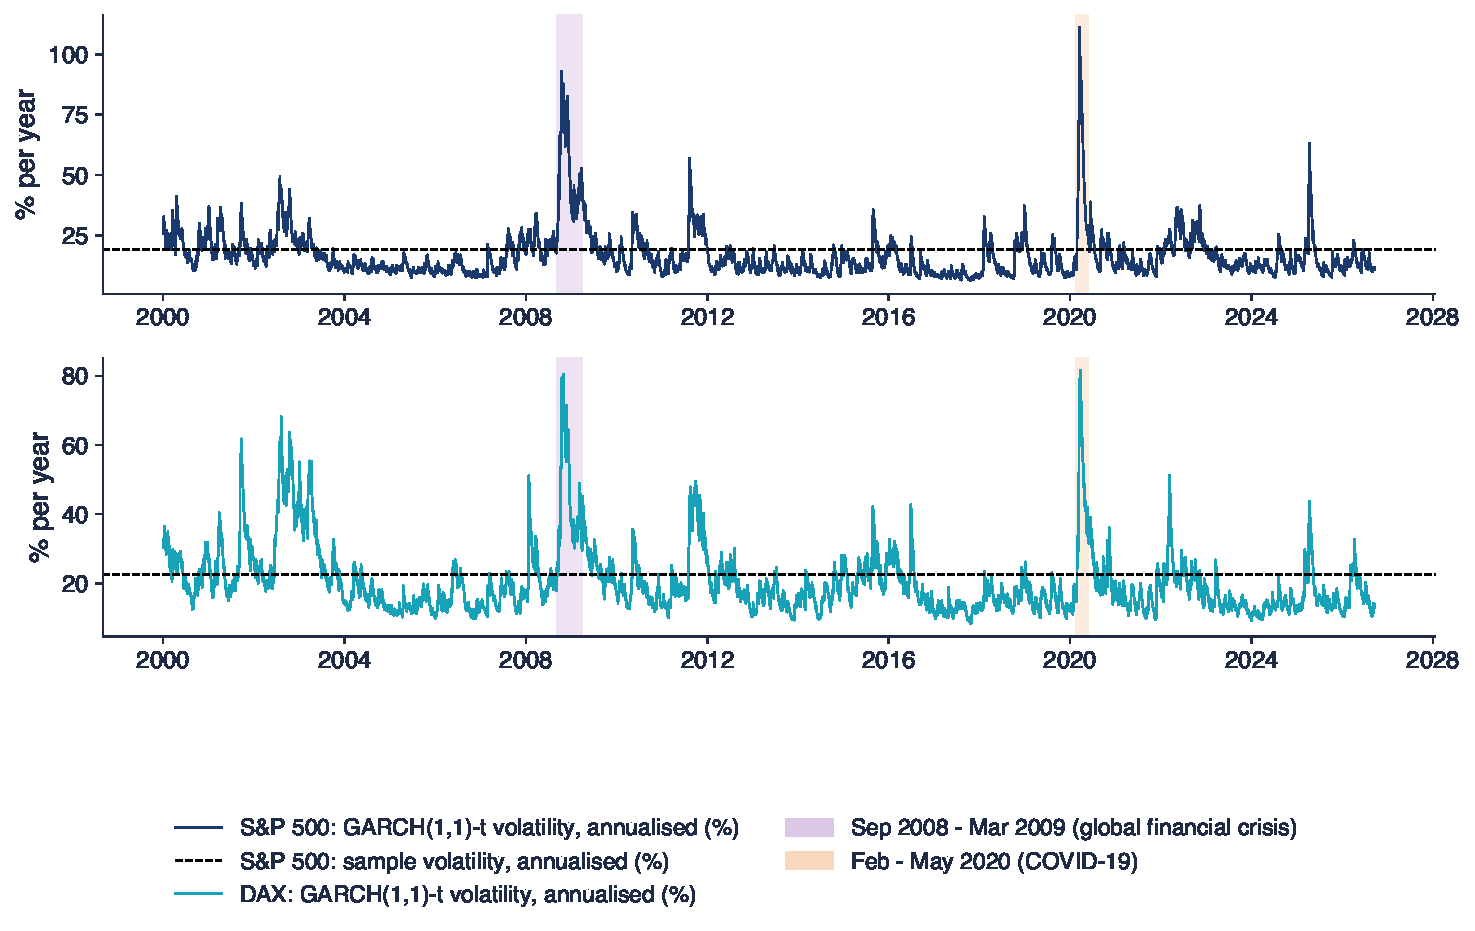
\includegraphics[width=0.97\textwidth,height=0.56\textheight,keepaspectratio]{sfm_ch9_vol_sp500_dax.pdf}
\end{center}
\vspace{-0.25cm}
\begin{itemize}
    \item GARCH(1,1)-t volatility $\hat\sigma_t$, annualised, as in SFEvolgarchest; dashed: the sample volatility
    \item S\&P 500: peaks 93\% (16 October 2008) and 111\% (17 March 2020); median 14\%; on 18 September 2026: 12\%
\end{itemize}
\sfmquantlet{Ch_09}{SFM_ch9_volatility_markets}
\end{frame}

\begin{frame}{Conditional Volatility: BET and Bitcoin}
\itemsize{\footnotesize}
\begin{center}
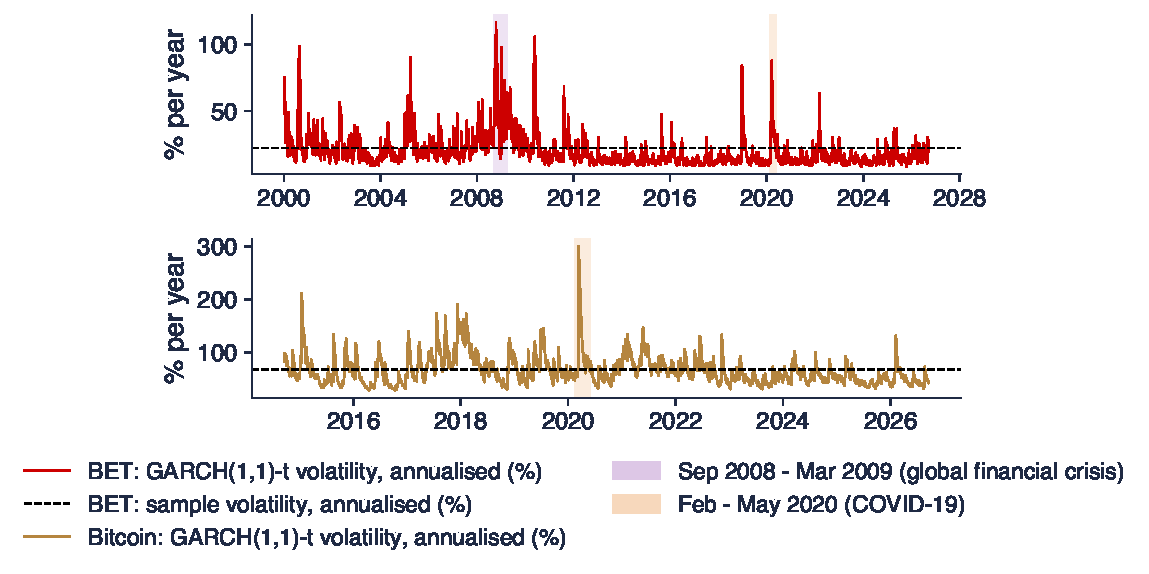
\includegraphics[width=0.97\textwidth,height=0.56\textheight,keepaspectratio]{sfm_ch9_vol_bet_btc.pdf}
\end{center}
\vspace{-0.25cm}
\begin{itemize}
    \item BET: the highest peak in 2008 (117\%, 15 October 2008), lower in 2020 (88\%); Bitcoin: 301\% on 13 March 2020, median 59\%
    \item Interpretation: the 2020 shock hit all markets in the same week; the median volatility of Bitcoin is 4.1 times that of the S\&P 500 (14\%)
\end{itemize}
\sfmquantlet{Ch_09}{SFM_ch9_volatility_markets}
\end{frame}

\begin{frame}{How Long Does a Shock Last?}
\itemsize{\footnotesize}
\begin{center}
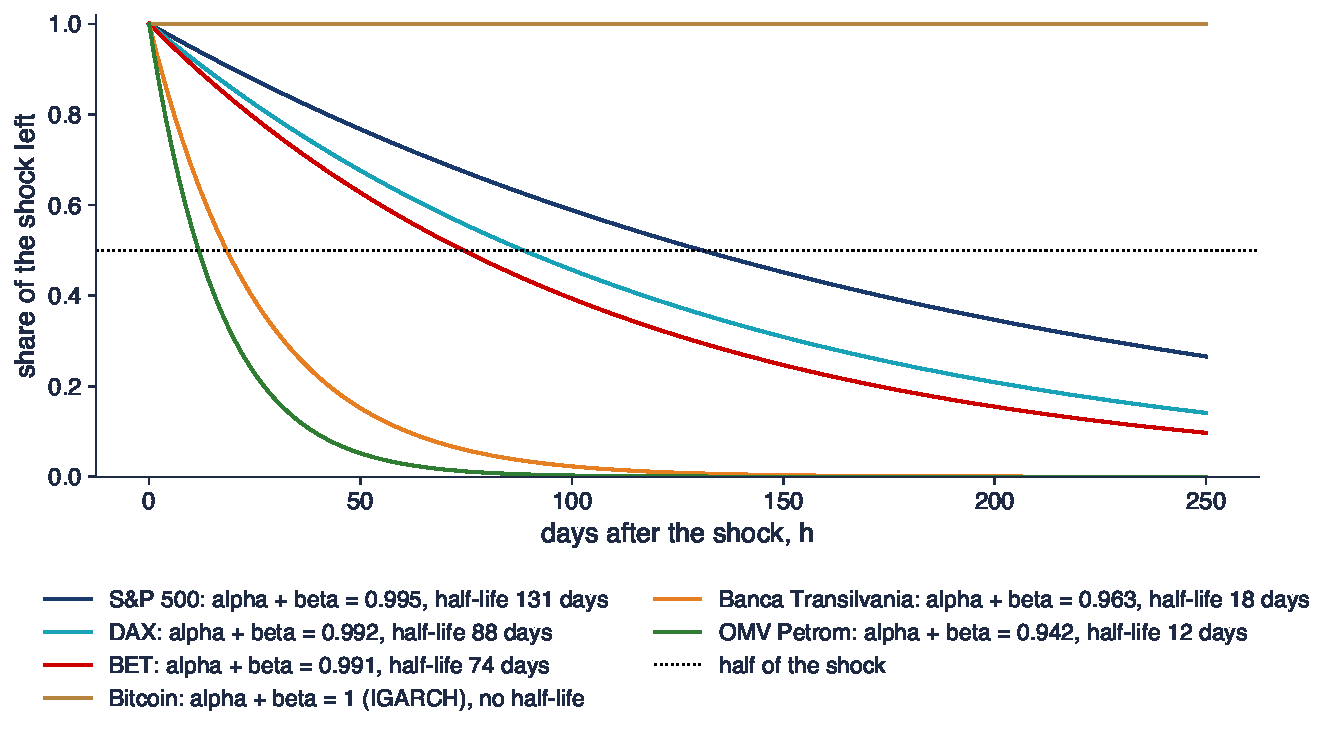
\includegraphics[width=0.97\textwidth,height=0.52\textheight,keepaspectratio]{sfm_ch9_persistence.pdf}
\end{center}
\vspace{-0.25cm}
\begin{itemize}
    \item Share of a variance shock left after $h$ days: $(\alpha + \beta)^h$; the half-life is where the curve crosses 1/2
    \item Interpretation: after a crisis, the S\&P 500 needs about half a year to halve the excess variance; OMV Petrom about two weeks; Bitcoin never
\end{itemize}
\sfmquantlet{Ch_09}{SFM_ch9_volatility_markets}
\end{frame}

\begin{frame}{Recap: GARCH in Six Markets}
\itemsize{\small}
\begin{itemize}
    \item $\alpha + \beta$ close to 1 everywhere: volatility shocks last for months
    \item BVB stocks: faster decay; Bitcoin: IGARCH, extreme tails
    \item The long-run volatility is imprecise when $\alpha + \beta$ is near 1
\end{itemize}
\end{frame}


%=============================================================================
\section{Asymmetry and the Leverage Effect}
%=============================================================================

\begin{frame}{The Leverage Effect}
\itemsize{\small}
\begin{itemize}
    \item Falls in stock prices are followed by larger increases in volatility than rises of the same size \refChristie
    \begin{itemize}
        \item \textbf{leverage} explanation: a lower share price raises the debt-to-equity ratio, so the equity becomes riskier
        \item \textbf{volatility feedback}: news of higher risk lowers prices at once
    \end{itemize}
    \item GARCH(1,1) cannot see it: $\sigma_t^2$ depends on $\varepsilon_{t-1}^2$, not on the sign of $\varepsilon_{t-1}$
    \begin{itemize}
        \item the QQ plot of Section 6 and the skewed t ($\hat\lambda < 0$) already pointed to the left tail
    \end{itemize}
    \item \textbf{NIC} (news impact curve) \refEN: $\sigma_t^2$ as a function of $\varepsilon_{t-1}$, with $\sigma_{t-1}^2$ fixed at the unconditional variance
\end{itemize}
\end{frame}

\begin{frame}{GJR-GARCH and EGARCH}
\itemsize{\small}
\begin{itemize}
    \item \textbf{GJR-GARCH} \refGJR: $\sigma_t^2 = \omega + (\alpha + \gamma\,I_{t-1})\,\varepsilon_{t-1}^2 + \beta\sigma_{t-1}^2$, $I_{t-1} = 1$ if $\varepsilon_{t-1} < 0$, else 0
    \begin{itemize}
        \item $I_{t-1}$: an indicator of a negative shock yesterday; $\gamma$: the extra reaction to bad news
        \item good news: slope $\alpha$; bad news: $\alpha + \gamma$; leverage effect: $\gamma > 0$
        \item persistence $\alpha + \beta + \gamma/2$ for symmetric $z_t$ (half of the shocks are negative)
    \end{itemize}
    \item \textbf{EGARCH} (exponential GARCH) \refNelson: $\ln\sigma_t^2 = \omega + \alpha\big(|z_{t-1}| - E|z_{t-1}|\big) + \gamma z_{t-1} + \beta\ln\sigma_{t-1}^2$
    \begin{itemize}
        \item $|z_{t-1}| - E|z_{t-1}|$: the size of yesterday's standardised shock above its average ($E|z| = \sqrt{2/\pi}$ for Normal $z$)
        \item the logarithm keeps $\sigma_t^2 > 0$ without sign restrictions on the parameters
        \item leverage effect: $\gamma < 0$ (a negative $z_{t-1}$ raises $\ln\sigma_t^2$); persistence: $\beta$
    \end{itemize}
    \item Textbook treatment of both, and of the threshold GARCH: \refFHH, Section 13.2
\end{itemize}
\end{frame}

\begin{frame}{News Impact Curves: S\&P 500 and Bitcoin}
\itemsize{\footnotesize}
\begin{center}
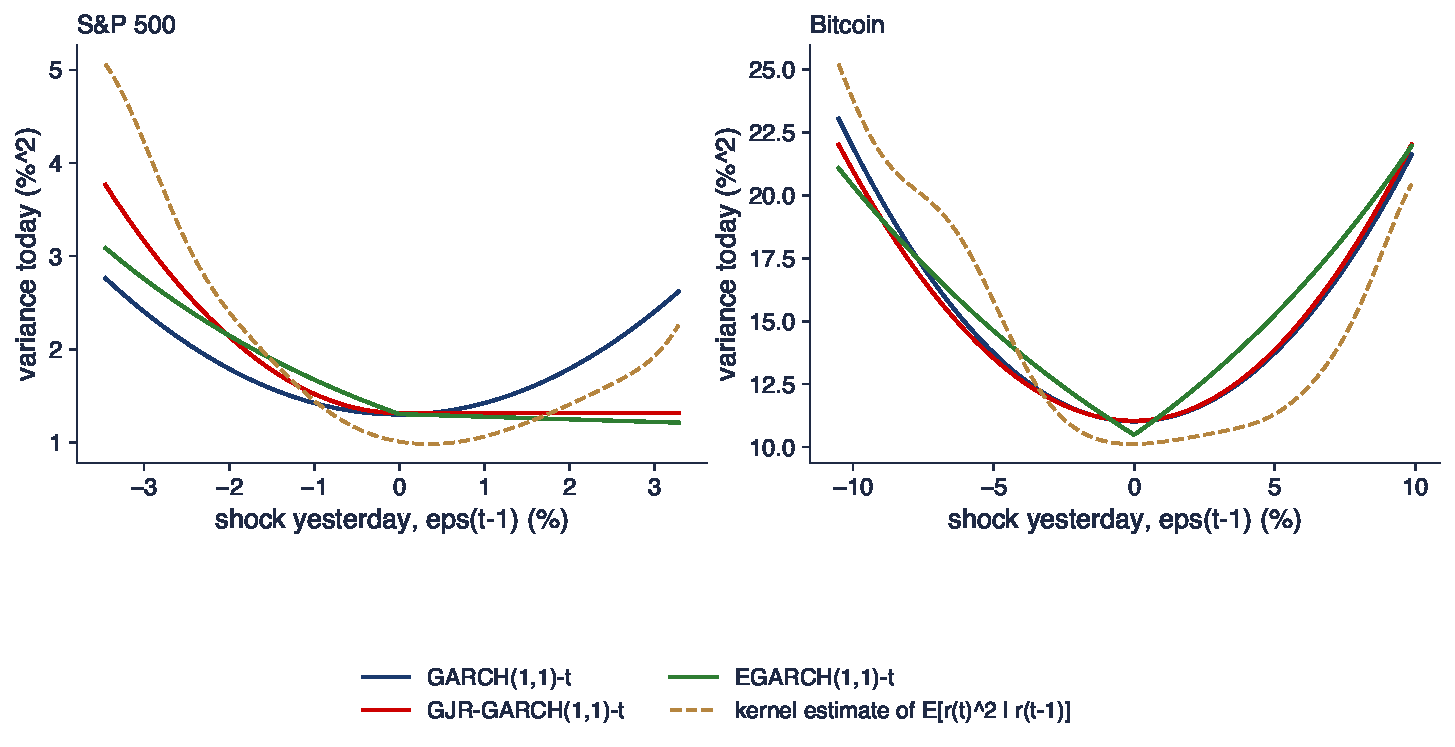
\includegraphics[width=0.97\textwidth,height=0.50\textheight,keepaspectratio]{sfm_ch9_nic.pdf}
\end{center}
\vspace{-0.25cm}
\begin{itemize}
    \item Model curves: $\sigma_t^2$ against $\varepsilon_{t-1}$, $\sigma_{t-1}^2$ fixed at the sample variance; dashed: a kernel (Nadaraya--Watson) estimate of $E[r_t^2 \mid r_{t-1}]$, the idea of SFENewsImpactCurve
    \item S\&P 500, GJR: after a fall of 2\%, tomorrow's variance is 1.62 times the variance after a rise of 2\%; Bitcoin: ratio 1.00, a symmetric curve
\end{itemize}
\sfmquantlet{Ch_09}{SFM_ch9_asymmetry}
\end{frame}

\begin{frame}{Asymmetry in Six Markets}
\itemsize{\footnotesize}
\begin{center}
\scriptsize
\begin{tabular}{lrrrrrrr}
\toprule
& GJR $\alpha$ & GJR $\gamma$ & $t(\gamma)$ & LR & p & EGARCH $\gamma$ & $t(\gamma)$ \\
\midrule
S\&P 500 & $0.000$ & $0.205$ & $10.0$ & $235.7$ & $<$\,0.001 & ${-0.165}$ & ${-15.2}$ \\
DAX & $0.000$ & $0.163$ & $8.7$ & $204.5$ & $<$\,0.001 & ${-0.133}$ & ${-11.8}$ \\
BET & $0.172$ & $0.043$ & $2.1$ & $4.9$ & 0.026 & ${-0.028}$ & ${-2.6}$ \\
Bitcoin & $0.113$ & $-0.013$ & $-0.7$ & $0.7$ & 0.416 & ${0.015}$ & ${1.2}$ \\
TLV & $0.101$ & $0.065$ & $2.7$ & $7.8$ & 0.005 & ${-0.040}$ & ${-3.0}$ \\
SNP & $0.117$ & $0.033$ & $1.4$ & $1.7$ & 0.188 & ${-0.027}$ & ${-1.9}$ \\
\bottomrule
\end{tabular}
\end{center}
\begin{itemize}
    \item Student-t innovations; $t$ statistics with robust SE; LR (likelihood ratio) $= 2(\ell_{GJR} - \ell_{GARCH}) \sim \chi^2(1)$
    \item S\&P 500 and DAX: GJR $\hat\alpha = 0$: only bad news raises volatility; a very strong leverage effect
    \item BET and TLV: a weak effect, significant by LR, yet BIC prefers the symmetric GARCH; SNP: not significant at 5\%; Bitcoin: none (EGARCH $\gamma$ slightly positive, not significant)
    \item Interpretation: leverage is a property of mature equity markets; in crypto, large rises are as ``frightening'' as large falls
\end{itemize}\sfmquantlet{Ch_09}{SFM_ch9_asymmetry}
\end{frame}

\begin{frame}{Recap: Asymmetry and the Leverage Effect}
\itemsize{\small}
\begin{itemize}
    \item GJR: an extra slope $\gamma$ for negative shocks; EGARCH: a sign term $\gamma z_{t-1}$ in $\ln\sigma_t^2$
    \item The news impact curve shows the asymmetry at a glance
    \item Strong in the S\&P 500 and the DAX, weak on the BVB, absent in Bitcoin
\end{itemize}
\end{frame}


%=============================================================================
\section{Diagnostics}
%=============================================================================

\begin{frame}{Checking a Fitted Model}
\itemsize{\small}
\begin{itemize}
    \item If the model is right, the \textbf{standardised residuals} $\hat z_t = (r_t - \hat\mu)/\hat\sigma_t$ are close to i.i.d.\ with mean 0 and variance 1
    \begin{itemize}
        \item \textbf{LB} (Ljung--Box) $Q(10)$ on $\hat z_t$: no autocorrelation left in the mean (\sfmchlink{https://danpele.github.io/SFM/EN/Courses/chapter7_efficient_markets_random_walk_vr.pdf}{Chapter 7}) \refLjung
        \item $Q(10)$ on $\hat z_t^2$ and the ARCH-LM test: no ARCH effects left (\sfmchlink{https://danpele.github.io/SFM/EN/Courses/chapter8_volatility_estimators.pdf}{Chapter 8})
        \item QQ plot of $\hat z_t$: is the assumed distribution right? (Section 6)
    \end{itemize}
    \item \textbf{Sign-bias test} \refEN: regress $\hat z_t^2$ on $I_{t-1}$, $I_{t-1}\hat\varepsilon_{t-1}$ and $(1 - I_{t-1})\hat\varepsilon_{t-1}$
    \begin{itemize}
        \item joint test $T R^2 \sim \chi^2(3)$: a rejection means the sign of past shocks still predicts the variance (asymmetry is missing)
    \end{itemize}
    \item A passed diagnostic does not prove the model right; a failed one shows where it is wrong
\end{itemize}
\end{frame}

\begin{frame}{What GARCH Removes}
\itemsize{\footnotesize}
\begin{center}
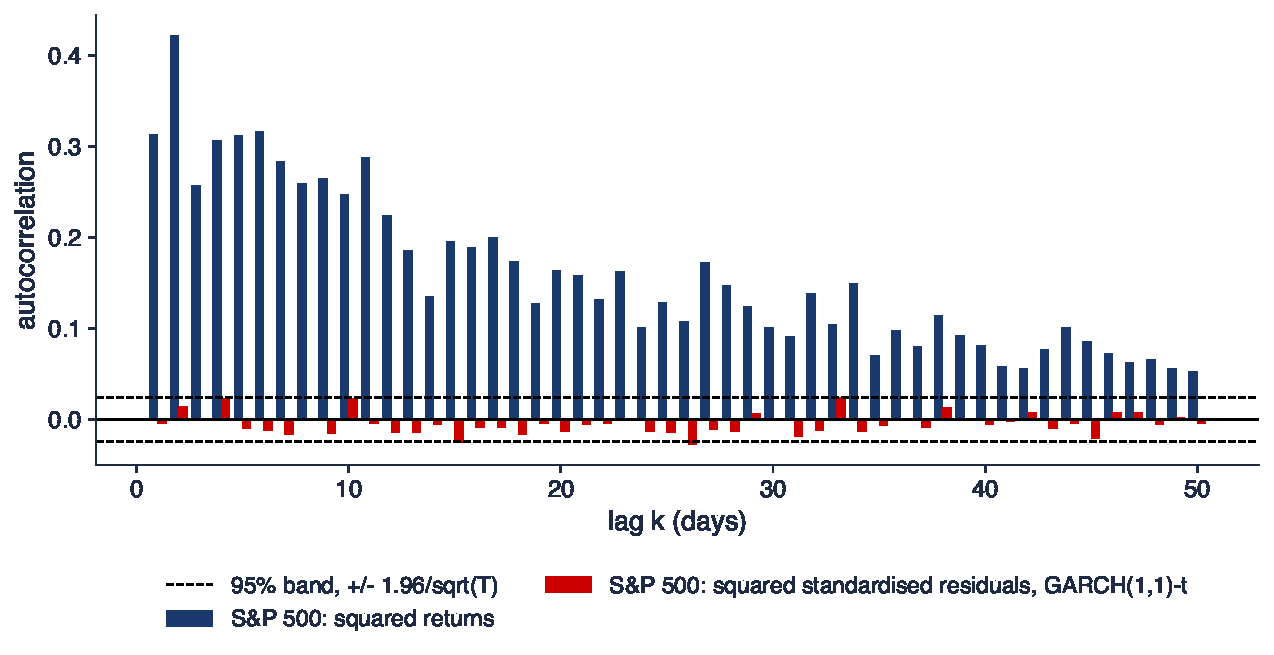
\includegraphics[width=0.97\textwidth,height=0.50\textheight,keepaspectratio]{sfm_ch9_acf_diag.pdf}
\end{center}
\vspace{-0.25cm}
\begin{itemize}
    \item ACF of $r_t^2$: $0.31$ at lag 1 and still $0.053$ at lag 50; ACF of $\hat z_t^2$ (GARCH(1,1)-t): $-0.005$ at lag 1, at most $0.028$ in absolute value; band $\pm0.024$
    \item Interpretation: three parameters absorb almost all the volatility clustering in the daily data since 2000
\end{itemize}
\sfmquantlet{Ch_09}{SFM_ch9_diagnostics}
\end{frame}

\begin{frame}{Diagnostics on Real Data}
\itemsize{\footnotesize}
\begin{center}
\scriptsize
\begin{tabular}{lrrrr}
\toprule
S\&P 500 & $Q(10)$ (p) & $Q(10)$ of squares (p) & ARCH-LM(5) (p) & sign bias $\chi^2(3)$ (p) \\
\midrule
returns $r_t$ & $96.3$ ($<$\,0.001) & $6133$ ($<$\,0.001) & $1679$ ($<$\,0.001) & -- \\
$\hat z_t$, Normal GARCH & $21.2$ (0.020) & $16.4$ (0.089) & $8.0$ (0.154) & -- \\
$\hat z_t$, GARCH-t & $21.9$ (0.016) & $13.6$ (0.192) & $5.8$ (0.326) & $40.7$ ($<$\,0.001) \\
\bottomrule
\end{tabular}
\end{center}
\begin{itemize}
    \item GARCH removes the ARCH effects ($Q(10)$ of squares: from $6133$ to $13.6$); a little autocorrelation in the mean remains (constant-mean model)
    \item The sign-bias test rejects for the symmetric GARCH (sign $t = 3.56$): the asymmetry of Section 8 is missing; similar for the DAX (p $<$\,0.001) and the BET (p = 0.009)
    \item Other markets, $Q(10)$ of $\hat z_t^2$ (GARCH-t): p between 0.115 (DAX) and 0.993 (TLV): no ARCH effect left anywhere
\end{itemize}\sfmquantlet{Ch_09}{SFM_ch9_diagnostics}
\end{frame}

\begin{frame}{Recap: Diagnostics}
\itemsize{\small}
\begin{itemize}
    \item Standardised residuals: no autocorrelation in $\hat z_t$ and $\hat z_t^2$, the right distribution
    \item GARCH(1,1)-t removes the ARCH effects in all six series
    \item The sign-bias test points to the missing asymmetry for equity indices
\end{itemize}
\end{frame}


%=============================================================================
\section{Model Selection}
%=============================================================================

\begin{frame}{Nine Models for the S\&P 500}
\itemsize{\footnotesize}
\begin{itemize}
    \item \textbf{AIC} (Akaike information criterion) $= -2\ell + 2k$ \refAkaike; \textbf{BIC} (Bayesian information criterion) $= -2\ell + k\ln T$ \refSchwarz; $\ell$: maximised log-likelihood, $k$ parameters, $T$ observations; smaller is better (\sfmchlink{https://danpele.github.io/SFM/EN/Courses/chapter6_model_selection_risk_management.pdf}{Chapter 6})
\end{itemize}\begin{center}
\scriptsize
\begin{tabular}{lrrrrrr}
\toprule
& \multicolumn{2}{c}{Normal} & \multicolumn{2}{c}{Student-t} & \multicolumn{2}{c}{skewed t} \\ & log-lik. & $\Delta$BIC & log-lik. & $\Delta$BIC & log-lik. & $\Delta$BIC \\
\midrule
GARCH(1,1) & \ensuremath{-}9218.0 & 648.9 & \ensuremath{-}9062.5 & 346.7 & \ensuremath{-}9038.4 & 307.4 \\
GJR-GARCH(1,1) & \ensuremath{-}9086.5 & 394.7 & \ensuremath{-}8944.6 & 119.9 & \ensuremath{-}8905.1 & 49.6 \\
EGARCH(1,1) & \ensuremath{-}9075.6 & 372.9 & \ensuremath{-}8922.1 & 74.8 & \ensuremath{-}8880.3 & 0.0 \\
\bottomrule
\end{tabular}
\end{center}
\begin{itemize}
    \item $\Delta$BIC: the difference from the best model; AIC gives the same ranking
    \item Both choices matter: starting from the Normal GARCH, asymmetry alone (Normal EGARCH) lowers BIC by 276, heavy tails alone (GARCH-skewed t) by 341, both together by 649
    \item Interpretation: EGARCH with skewed-t innovations wins; with 6\,714 observations even small improvements are ``significant''; the forecast comparison in Section 11 is the real test
\end{itemize}\sfmquantlet{Ch_09}{SFM_ch9_diagnostics}
\end{frame}

\begin{frame}{Recap: Model Selection}
\itemsize{\small}
\begin{itemize}
    \item Compare models fitted on the same data with AIC/BIC; BIC penalises parameters more
    \item S\&P 500: asymmetry and heavy tails both needed; EGARCH-skewed t is the best
    \item In-sample fit is not forecasting ability
\end{itemize}
\end{frame}


%=============================================================================
\section{Volatility Forecasts}
%=============================================================================

\begin{frame}{Multi-Step Forecasts}
\itemsize{\small}
\begin{itemize}
    \item One step: $\sigma_{t+1}^2 = \omega + \alpha\varepsilon_t^2 + \beta\sigma_t^2$ is known at the end of day $t$
    \begin{itemize}
        \item two steps: $E_t[\sigma_{t+2}^2] = \omega + \alpha E_t[\varepsilon_{t+1}^2] + \beta\sigma_{t+1}^2 = \omega + (\alpha + \beta)\sigma_{t+1}^2$, since $E_t[\varepsilon_{t+1}^2] = \sigma_{t+1}^2$
    \end{itemize}
    \item By induction: $E_t[\sigma_{t+h}^2] = \bar\sigma^2 + (\alpha + \beta)^{h-1}(\sigma_{t+1}^2 - \bar\sigma^2)$
    \begin{itemize}
        \item $E_t$: the expectation given the information at the end of day $t$; $h$: the horizon in days
        \item the forecast converges to the long-run variance; the speed is set by $\alpha + \beta$
    \end{itemize}
    \item Variance of the $H$-day return: the sum of the daily forecasts (returns are uncorrelated)
    \begin{itemize}
        \item $\mathrm{Var}_t(r_{t+1} + \dots + r_{t+H}) = \sum_{h=1}^{H} E_t[\sigma_{t+h}^2]$, not $H\sigma_{t+1}^2$
        \item the square-root-of-time rule $\sigma_{t+1}\sqrt{H}$ is too high in a crisis and too low in a calm period
    \end{itemize}
\end{itemize}
\end{frame}

\begin{frame}{Worked Example: the S\&P 500 on 18 September 2026}
\itemsize{\small}
\begin{itemize}
    \item GARCH(1,1)-t: $\alpha + \beta = 0.9947$, $\bar\sigma^2 = 2.972$; forecast for the next day $\sigma_{t+1}^2 = 0.509$ (below the long-run level)
    \item Step by step
    \begin{itemize}
        \item day 10: $2.972 + 0.9947^{9}(0.509 - 2.972) = 2.972 + 0.953 \times (0.509 - 2.972) = 0.624$
        \item 10-day variance: the sum of the ten daily forecasts $= 5.67$, so the 10-day volatility is $2.38\%$
        \item square-root-of-time rule: $\sqrt{10 \times 0.509} = 2.26\%$: too low, because volatility is expected to rise towards its long-run level
    \end{itemize}
\end{itemize}
\end{frame}

\begin{frame}{The Term Structure of Volatility}
\itemsize{\footnotesize}
\begin{center}
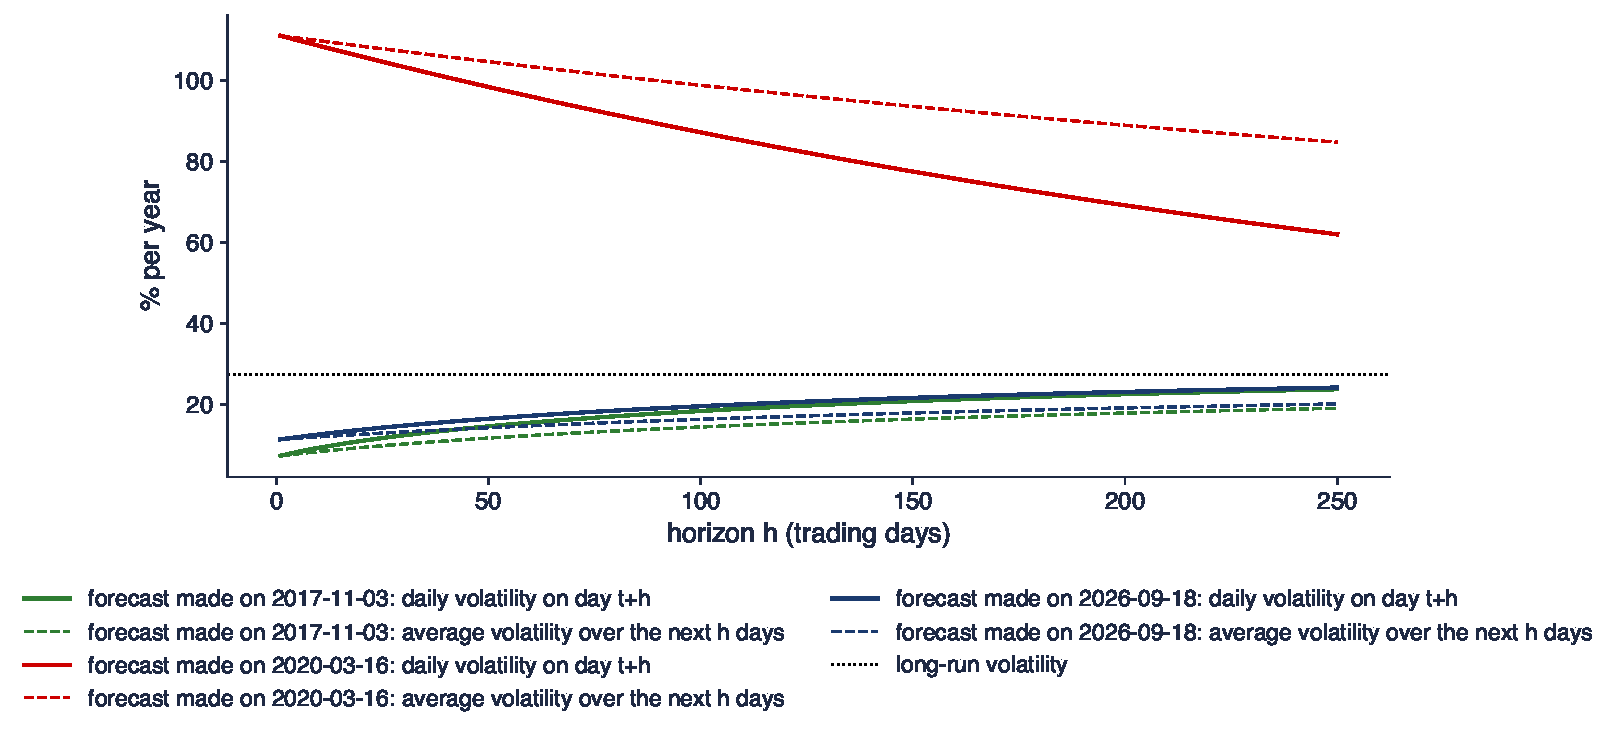
\includegraphics[width=0.97\textwidth,height=0.50\textheight,keepaspectratio]{sfm_ch9_term_structure.pdf}
\end{center}
\vspace{-0.25cm}
\begin{itemize}
    \item S\&P 500, GARCH(1,1)-t estimated on all data; forecasts made on a calm day (3 November 2017), at the COVID-19 peak (16 March 2020) and on 18 September 2026
    \item Calm day: 7.3\% tomorrow, average 19.0\% over a year; COVID-19 peak: 111.0\% tomorrow, still 84.7\% on average over a year
    \item Interpretation: all curves move towards the long-run level (27.3\%) at the same slow speed: the slope of the term structure tells whether we are in a calm or a storm
\end{itemize}
\sfmquantlet{Ch_09}{SFM_ch9_forecasts}
\end{frame}

\begin{frame}{How to Evaluate a Volatility Forecast}
\itemsize{\small}
\begin{itemize}
    \item The true $\sigma_t^2$ is never observed: we compare the forecast $h_t$ with a noisy \textbf{proxy}, here $r_t^2$
    \begin{itemize}
        \item $E_{t-1}[r_t^2] = \sigma_t^2$ (with $\mu \approx 0$), but $r_t^2$ is very noisy: low $R^2$ even for a perfect forecast \refAB
    \end{itemize}
    \item \textbf{QLIKE} loss \refPatton: $L(r_t^2, h_t) = \dfrac{r_t^2}{h_t} + \ln h_t$ (up to a constant); smaller is better
    \begin{itemize}
        \item $h_t$: the variance forecast for day $t$, made at the end of day $t-1$
        \item ranks forecasts correctly even with a noisy proxy; it is minus the Normal log-likelihood
        \item penalises forecasts that are too low more than forecasts that are too high
    \end{itemize}
    \item \textbf{Out of sample}: from 2015, each forecast uses only data up to the day before; the models are re-estimated every 250 days
    \begin{itemize}
        \item the \textbf{DM} (Diebold--Mariano) test \refDM: is the mean loss difference zero? $t$ with HAC (heteroskedasticity and autocorrelation consistent) standard errors
    \end{itemize}
\end{itemize}
\end{frame}

\begin{frame}{GARCH against EWMA, Out of Sample}
\itemsize{\scriptsize}
\begin{center}
\scriptsize
\begin{tabular}{lrrrrr}
\toprule
2015--2026 & days & QLIKE GARCH-t & QLIKE GJR-t & QLIKE EWMA & DM $t$, GARCH-t vs EWMA (p) \\
\midrule
S\&P 500 & 2\,944 & $0.761$ & $0.733$ & $0.819$ & ${-3.69}$ ($<$\,0.001) \\
DAX & 2\,973 & $1.090$ & $1.064$ & $1.121$ & ${-3.19}$ (0.001) \\
BET & 2\,926 & $0.680$ & $0.674$ & $0.788$ & ${-2.22}$ (0.027) \\
Bitcoin & 4\,279 & $3.383$ & $3.401$ & $3.390$ & ${-0.20}$ (0.845) \\
\bottomrule
\end{tabular}
\end{center}
\vspace{-1mm}
\begin{center}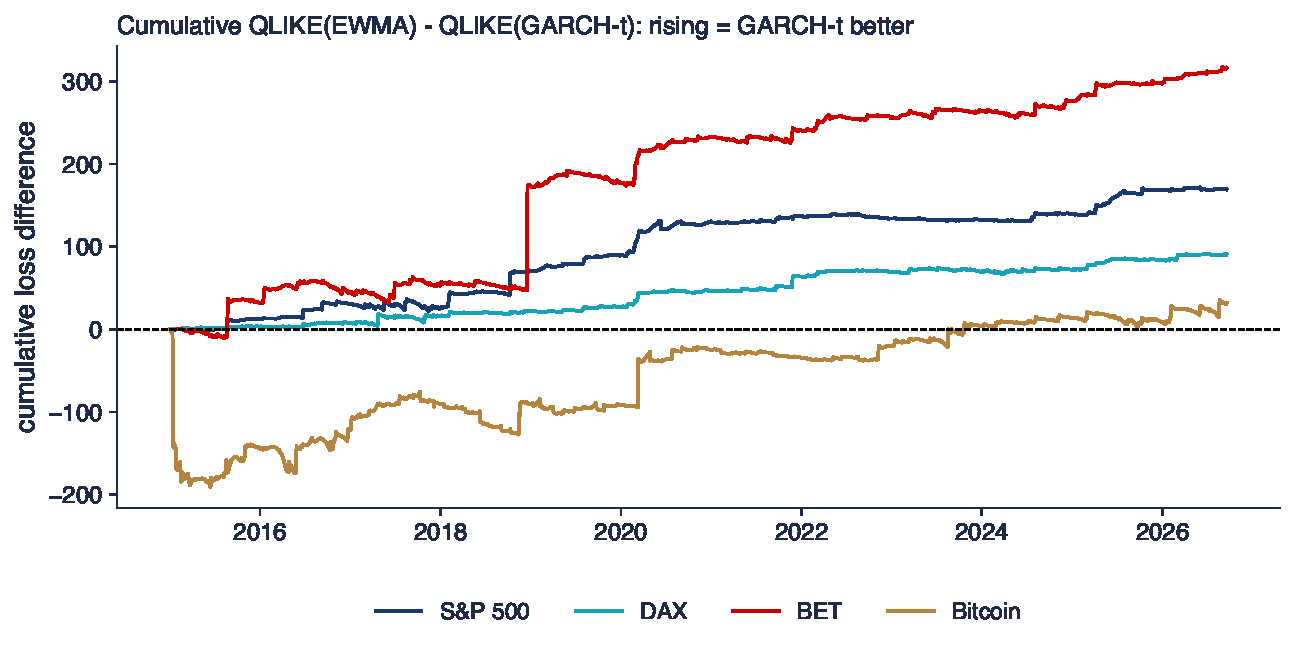
\includegraphics[width=0.80\textwidth,height=0.34\textheight,keepaspectratio]{sfm_ch9_forecast_eval.pdf}\end{center}
\vspace{-3mm}
\begin{itemize}
    \item Equity indices: GARCH-t beats EWMA ($t < -2$); GJR-t is better still for the S\&P 500, DAX and BET
    \item Interpretation: Bitcoin: no difference ($t = -0.20$): its GARCH is an IGARCH, which is almost an EWMA (Section 7)
\end{itemize}\sfmquantlet{Ch_09}{SFM_ch9_forecasts}
\end{frame}

\begin{frame}{Recap: Volatility Forecasts}
\itemsize{\small}
\begin{itemize}
    \item $E_t[\sigma_{t+h}^2] = \bar\sigma^2 + (\alpha + \beta)^{h-1}(\sigma_{t+1}^2 - \bar\sigma^2)$; $H$-day variance = sum of daily forecasts
    \item Compare forecasts out of sample with QLIKE and the Diebold--Mariano test
    \item GARCH beats EWMA where volatility mean-reverts
\end{itemize}
\end{frame}


%=============================================================================
\section{VaR 1\% from a GARCH Model}
%=============================================================================

\begin{frame}{Conditional VaR}
\itemsize{\small}
\begin{itemize}
    \item \textbf{VaR} at level $\alpha$ (value at risk): the loss exceeded with probability $\alpha$: $\mathrm{VaR}_\alpha = -q_\alpha(r_{t+1})$ (\sfmchlink{https://danpele.github.io/SFM/EN/Courses/chapter6_model_selection_risk_management.pdf}{Chapter 6})
    \begin{itemize}
        \item here $\alpha$ is the VaR level, not the GARCH parameter; $q_\alpha$: the $\alpha$-quantile
        \item here $\alpha = 1\%$: VaR 1\%, a loss exceeded on one day in a hundred
    \end{itemize}
    \item With $r_{t+1} = \mu + \sigma_{t+1}z_{t+1}$: $\mathrm{VaR}_{t+1} = -(\mu + \sigma_{t+1}\,q_\alpha(z))$
    \begin{itemize}
        \item Normal: $q_{0.01} = -2.326$; standardised t: $q_{0.01} = t_\nu^{-1}(0.01)\sqrt{(\nu - 2)/\nu}$
        \item $t_\nu^{-1}(0.01)$: the 1\% quantile of the Student-t with $\nu$ degrees of freedom; the square root rescales it to variance 1
        \item the VaR moves every day with $\sigma_{t+1}$: high in storms, low in calm periods
    \end{itemize}
    \item \textbf{Worked example}: S\&P 500 on 18 September 2026, GARCH(1,1)-t: $\hat\mu = 0.079$, $\sigma_{t+1} = 0.714$, $\hat\nu = 6.26$
    \begin{itemize}
        \item $q_{0.01}(z) = -3.100 \times 0.825 = -2.557$; VaR 1\% $= -(0.079 + 0.714 \times (-2.557)) = 1.75\%$
        \item with Normal $z_t$: $1.58\%$; over 10 days (sum of variances, $\mu$ ignored): $2.557 \times \sqrt{5.67}$, about $6.09\%$
    \end{itemize}
\end{itemize}
\end{frame}

\begin{frame}{VaR 1\% through the COVID-19 Crash}
\itemsize{\footnotesize}
\begin{center}
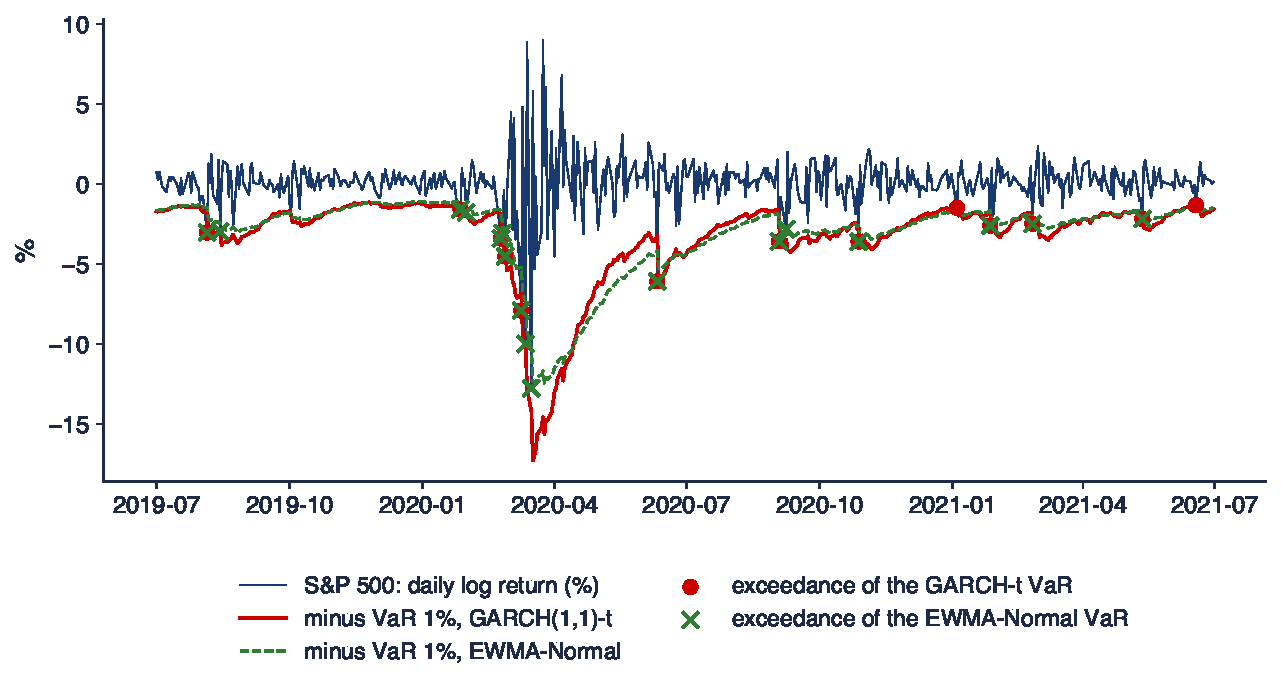
\includegraphics[width=0.97\textwidth,height=0.50\textheight,keepaspectratio]{sfm_ch9_var.pdf}
\end{center}
\vspace{-0.25cm}
\begin{itemize}
    \item S\&P 500, July 2019 -- June 2021 (505 days): one-day VaR 1\% from GARCH(1,1)-t (re-estimated every 250 days) and from EWMA with Normal $z_t$
    \item Exceedances (return below $-$VaR): GARCH-t 13, EWMA-Normal 17; expected about 5; both models react, but only after the first large falls of March 2020
\end{itemize}
\sfmquantlet{Ch_09}{SFM_ch9_forecasts}
\end{frame}

\begin{frame}{Exceedances 2015--2026: a Preview of Backtesting}
\itemsize{\footnotesize}
\begin{center}
\footnotesize
\begin{tabular}{lrrrr}
\toprule
VaR 1\% & days & expected & GARCH-t & EWMA-Normal \\
\midrule
S\&P 500 & 2\,944 & 29 & 49 (1.66\%) & 65 (2.21\%) \\
DAX & 2\,973 & 30 & 45 (1.51\%) & 74 (2.49\%) \\
BET & 2\,926 & 29 & 34 (1.16\%) & 67 (2.29\%) \\
Bitcoin & 4\,279 & 43 & 64 (1.50\%) & 93 (2.17\%) \\
\bottomrule
\end{tabular}
\end{center}
\begin{itemize}
    \item A correct VaR 1\% is exceeded on 1\% of the days, and the exceedances do not cluster
    \item EWMA-Normal: 2.2--2.5\%: the Normal quantile is too small for heavy tails
    \item GARCH-t: 1.2--1.7\%: much closer to 1\%, but still above it for the S\&P 500 and the DAX (the leverage effect is missing)
    \item Are these differences significant? \sfmchlink{https://danpele.github.io/SFM/EN/Courses/chapter10_var_es_backtesting.pdf}{Chapter 10}: the test of \refKupiec, ES 2.5\%, backtesting
    \item Further reading on VaR forecasting for Bitcoin: \refPeleB
\end{itemize}\sfmquantlet{Ch_09}{SFM_ch9_forecasts}
\end{frame}

\begin{frame}{Recap: VaR 1\% from a GARCH Model}
\itemsize{\small}
\begin{itemize}
    \item $\mathrm{VaR}_{t+1} = -(\mu + \sigma_{t+1}q_\alpha(z))$: dynamic volatility and the right quantile
    \item Normal quantiles underestimate the risk; Student-t is much closer to 1\%
    \item Formal backtests: \sfmchlink{https://danpele.github.io/SFM/EN/Courses/chapter10_var_es_backtesting.pdf}{Chapter 10}
\end{itemize}
\end{frame}


%=============================================================================
\section{AI for Scientific Discovery}
%=============================================================================

\begin{frame}{An Open Question}
\itemsize{\small}
\begin{itemize}
    \item \textbf{Is Bitcoin's volatility becoming more like the volatility of an equity index?}
    \begin{itemize}
        \item today: IGARCH, $\hat\nu = 3.18$, no leverage effect; the S\&P 500: mean-reverting, strong leverage
        \item since 2024, spot Bitcoin ETFs (exchange-traded funds) bring equity investors to the crypto market
    \end{itemize}
    \item Earlier evidence on crypto assets as an asset class: \refPeleC; volatility as information: \refPeleA
    \item Why it is open: regime changes, the 2022 crypto crash and the ETF launch overlap; the answer depends on the window
    \item AI tools can speed up such a study, but its results must still be checked \refWang
\end{itemize}
\end{frame}

\begin{frame}{How AI Could Help}
\itemsize{\small}
\begin{itemize}
    \item \textbf{Literature}: a list of studies on GARCH models for crypto assets and the models they use
    \item \textbf{Code}: a first draft of rolling GJR-GARCH-t estimates for Bitcoin and the S\&P 500 with the \texttt{arch} package
    \item \textbf{Robustness}: other windows, Ethereum, weekend days removed, skewed-t innovations
    \item Example prompt
    \begin{itemize}
        \item \aiprompt{Write Python code that estimates a GJR-GARCH(1,1) model with Student-t innovations on daily Bitcoin and S\&P 500 log returns in percent, on rolling windows of 750 days moved by 21 days, and plots the persistence, gamma and nu over time.}
    \end{itemize}
\end{itemize}
\end{frame}

\begin{frame}{What to Check}
\itemsize{\small}
\begin{itemize}
    \item Units: returns in \% (not decimals), otherwise the optimiser may stop at a wrong $\omega$
    \item The persistence of GJR is $\alpha + \beta + \gamma/2$, not $\alpha + \beta$; for EGARCH it is $\beta$
    \item Estimates on the boundary ($\alpha + \beta = 1$): no half-life, no long-run volatility; do not report infinite numbers
    \item Calendars: Bitcoin trades 7 days a week, the S\&P 500 five; annualise each series with its own frequency
    \item Rolling windows overlap: consecutive estimates are not independent evidence
    \item References: every cited paper must exist; check the DOI
\end{itemize}
\end{frame}

\begin{frame}{Project Idea}
\itemsize{\small}
\begin{itemize}
    \item \textbf{Question}: has Bitcoin's volatility moved closer to equity volatility since 2021?
    \begin{itemize}
        \item data: Bitcoin since 2014, Ethereum since 2015, S\&P 500 and BET (EODHD)
    \end{itemize}
    \item Steps
    \begin{itemize}
        \item GJR-GARCH-t on 2015--2019 and on 2021--2026: persistence, $\gamma$, $\nu$
        \item correlation of the Bitcoin and S\&P 500 GARCH volatilities in each period
        \item out-of-sample QLIKE of GARCH against EWMA in each period
    \end{itemize}
    \item Deliverable: one table, one chart, and a paragraph on what the data can and cannot show
    \item Declare any AI use, and list the errors of the AI that you corrected
\end{itemize}
\end{frame}


%=============================================================================
\section{Summary}
%=============================================================================

\begin{frame}{Key Takeaways}
\itemsize{\small}
\begin{itemize}
    \item Returns: unpredictable mean, predictable variance: $r_t = \mu + \sigma_t z_t$
    \item GARCH(1,1) with three parameters captures volatility clustering in all our series; $\alpha + \beta$ is close to 1
    \item Estimate by maximum likelihood, report robust SE; Student-t or skewed-t innovations for the tails
    \item Equity indices need asymmetry (GJR, EGARCH); Bitcoin does not, and is an IGARCH
    \item Forecasts revert to the long-run level; GARCH beats EWMA out of sample where volatility mean-reverts
    \item VaR 1\% = $-(\mu + \sigma_{t+1}q_{0.01}(z))$: the volatility model and the quantile both matter
\end{itemize}
\end{frame}

\begin{frame}{Key Formulas}
\itemsize{\small}
{\renewcommand{\arraystretch}{1.45}\begin{center}
\small
\begin{tabular}{ll}
\toprule
\textbf{Quantity} & \textbf{Formula} \\
\midrule
ARCH($q$) & $\sigma_t^2 = \omega + \sum_{i=1}^{q}\alpha_i\varepsilon_{t-i}^2$, \quad $\bar\sigma^2 = \omega/(1 - \sum\alpha_i)$ \\
GARCH(1,1) & $\sigma_t^2 = \omega + \alpha\varepsilon_{t-1}^2 + \beta\sigma_{t-1}^2$, \quad $\bar\sigma^2 = \omega/(1 - \alpha - \beta)$ \\
Half-life & $h_{1/2} = \ln 0.5/\ln(\alpha + \beta)$ \\
GJR-GARCH & $\sigma_t^2 = \omega + (\alpha + \gamma I_{t-1})\varepsilon_{t-1}^2 + \beta\sigma_{t-1}^2$ \\
EGARCH & $\ln\sigma_t^2 = \omega + \alpha(|z_{t-1}| - E|z_{t-1}|) + \gamma z_{t-1} + \beta\ln\sigma_{t-1}^2$ \\
Log-likelihood (Normal) & $\ell = -\frac12\sum_t[\ln 2\pi + \ln\sigma_t^2 + (r_t - \mu)^2/\sigma_t^2]$ \\
Forecast & $E_t[\sigma_{t+h}^2] = \bar\sigma^2 + (\alpha + \beta)^{h-1}(\sigma_{t+1}^2 - \bar\sigma^2)$ \\
QLIKE & $L = r_t^2/h_t + \ln h_t$ \\
VaR 1\% & $-(\mu + \sigma_{t+1}\,q_{0.01}(z))$ \\
\bottomrule
\end{tabular}
\end{center}
}
\end{frame}

\begin{frame}{Check Yourself}
\itemsize{\small}
\begin{itemize}
    \item \textbf{Question}: $\omega = 0.05$, $\alpha = 0.05$, $\beta = 0.90$. What are the long-run variance and the half-life?
    \begin{itemize}
        \item \textbf{Answer}: $0.05/0.05 = 1$; $\ln 0.5/\ln 0.95 = 13.5$ days
    \end{itemize}
    \item \textbf{Question}: GJR gives $\hat\alpha = 0$, $\hat\gamma = 0.2$. What happens after a rise of 3\%?
    \begin{itemize}
        \item \textbf{Answer}: nothing beyond the decay $\beta\sigma_t^2$: only negative shocks raise the variance
    \end{itemize}
    \item \textbf{Question}: $Q(10)$ of $\hat z_t^2$ has p $= 0.40$. Is the model correct?
    \begin{itemize}
        \item \textbf{Answer}: we only know that no ARCH effect is left; asymmetry or the wrong distribution may remain
    \end{itemize}
    \item Next: \sfmchlink{https://danpele.github.io/SFM/EN/Courses/chapter10_var_es_backtesting.pdf}{Chapter 10}, VaR, ES and backtesting
\end{itemize}
\end{frame}


%=============================================================================
\section{References}
%=============================================================================

\begin{frame}{References (1/2)}
\itemsize{\tiny}
\begin{itemize}
    \item Akaike, H. (1974). \href{https://doi.org/10.1109/TAC.1974.1100705}{A new look at the statistical model identification}. \textit{IEEE Transactions on Automatic Control}, 19(6), 716--723.
    \item Andersen, T.G., Bollerslev, T. (1998). \href{https://doi.org/10.2307/2527343}{Answering the skeptics: yes, standard volatility models do provide accurate forecasts}. \textit{International Economic Review}, 39(4), 885--905.
    \item Bollerslev, T. (1986). \href{https://doi.org/10.1016/0304-4076(86)90063-1}{Generalized autoregressive conditional heteroskedasticity}. \textit{Journal of Econometrics}, 31(3), 307--327.
    \item Bollerslev, T. (1987). \href{https://doi.org/10.2307/1925546}{A conditionally heteroskedastic time series model for speculative prices and rates of return}. \textit{Review of Economics and Statistics}, 69(3), 542--547.
    \item Bollerslev, T., Wooldridge, J.M. (1992). \href{https://doi.org/10.1080/07474939208800229}{Quasi-maximum likelihood estimation and inference in dynamic models with time-varying covariances}. \textit{Econometric Reviews}, 11(2), 143--172.
    \item Borak, S., Härdle, W.K., López-Cabrera, B. (2013). \href{https://doi.org/10.1007/978-3-642-33929-5}{\textit{Statistics of Financial Markets: Exercises and Solutions}}, 2nd ed. Springer.
    \item Christie, A.A. (1982). \href{https://doi.org/10.1016/0304-405X(82)90018-6}{The stochastic behavior of common stock variances: value, leverage and interest rate effects}. \textit{Journal of Financial Economics}, 10(4), 407--432.
    \item Diebold, F.X., Mariano, R.S. (1995). \href{https://doi.org/10.1080/07350015.1995.10524599}{Comparing predictive accuracy}. \textit{Journal of Business \& Economic Statistics}, 13(3), 253--263.
    \item Engle, R.F. (1982). \href{https://doi.org/10.2307/1912773}{Autoregressive conditional heteroscedasticity with estimates of the variance of United Kingdom inflation}. \textit{Econometrica}, 50(4), 987--1007.
    \item Engle, R.F. (2004). \href{https://doi.org/10.1257/0002828041464597}{Risk and volatility: econometric models and financial practice}. \textit{American Economic Review}, 94(3), 405--420.
    \item Engle, R.F., Bollerslev, T. (1986). \href{https://doi.org/10.1080/07474938608800095}{Modelling the persistence of conditional variances}. \textit{Econometric Reviews}, 5(1), 1--50.
    \item Engle, R.F., Ng, V.K. (1993). \href{https://doi.org/10.1111/j.1540-6261.1993.tb05127.x}{Measuring and testing the impact of news on volatility}. \textit{Journal of Finance}, 48(5), 1749--1778.
    \item Franke, J., Härdle, W.K., Hafner, C.M. (2019). \href{https://doi.org/10.1007/978-3-030-13751-9}{\textit{Statistics of Financial Markets: An Introduction}}, 5th ed. Springer.
\end{itemize}
\end{frame}

\begin{frame}{References (2/2)}
\itemsize{\tiny}
\begin{itemize}
    \item Glosten, L.R., Jagannathan, R., Runkle, D.E. (1993). \href{https://doi.org/10.1111/j.1540-6261.1993.tb05128.x}{On the relation between the expected value and the volatility of the nominal excess return on stocks}. \textit{Journal of Finance}, 48(5), 1779--1801.
    \item Hansen, B.E. (1994). \href{https://doi.org/10.2307/2527081}{Autoregressive conditional density estimation}. \textit{International Economic Review}, 35(3), 705--730.
    \item Hansen, P.R., Lunde, A. (2005). \href{https://doi.org/10.1002/jae.800}{A forecast comparison of volatility models: does anything beat a GARCH(1,1)?} \textit{Journal of Applied Econometrics}, 20(7), 873--889.
    \item Kupiec, P.H. (1995). \href{https://doi.org/10.3905/jod.1995.407942}{Techniques for verifying the accuracy of risk measurement models}. \textit{Journal of Derivatives}, 3(2), 73--84.
    \item Ljung, G.M., Box, G.E.P. (1978). \href{https://doi.org/10.1093/biomet/65.2.297}{On a measure of lack of fit in time series models}. \textit{Biometrika}, 65(2), 297--303.
    \item Nelson, D.B. (1991). \href{https://doi.org/10.2307/2938260}{Conditional heteroskedasticity in asset returns: a new approach}. \textit{Econometrica}, 59(2), 347--370.
    \item Patton, A.J. (2011). \href{https://doi.org/10.1016/j.jeconom.2010.03.034}{Volatility forecast comparison using imperfect volatility proxies}. \textit{Journal of Econometrics}, 160(1), 246--256.
    \item Pele, D.T., Lazar, E., Dufour, A. (2017). \href{https://doi.org/10.3390/e19050226}{Information entropy and measures of market risk}. \textit{Entropy}, 19(5), 226.
    \item Pele, D.T., Mazurencu-Marinescu-Pele, M. (2019). \href{https://doi.org/10.3390/e21020102}{Using high-frequency entropy to forecast Bitcoin's daily value at risk}. \textit{Entropy}, 21(2), 102.
    \item Pele, D.T., Wesselhöfft, N., Härdle, W.K., Kolossiatis, M., Yatracos, Y.G. (2023). \href{https://doi.org/10.1080/1351847x.2021.1960403}{Are cryptos becoming alternative assets?} \textit{European Journal of Finance}, 29(10), 1064--1105.
    \item Schwarz, G. (1978). \href{https://doi.org/10.1214/aos/1176344136}{Estimating the dimension of a model}. \textit{Annals of Statistics}, 6(2), 461--464.
    \item Tsay, R.S. (2010). \href{https://doi.org/10.1002/9780470644560}{\textit{Analysis of Financial Time Series}}, 3rd ed. Wiley.
    \item Wang, H., Fu, T., Du, Y., Gao, W., et al. (2023). \href{https://doi.org/10.1038/s41586-023-06221-2}{Scientific discovery in the age of artificial intelligence}. \textit{Nature}, 620, 47--60.
\end{itemize}
\end{frame}

\end{document}
